\chapter{Results and discussion}\label{chap:Results&Disc}
\section{PFCA sorption behavior}
\subsection{Biochar-water sorption isotherms}
\cref{fig:sorption_isotherms} shows the sorption isotherms for PFPeA, PFHxA, PFHpA, PFOA, PFNA and PFDA on CWC, ULS and DSL biochars. The points generated from the batch tests were fitted using the Freundlich model (\cref{eq:FreundlichLinear}). For all compounds, the sorption isotherm for ULS was visibly higher than DSL, followed by CWC. The Freundlich sorption coefficients ($\log~K_F$), linearity coefficients ($n_F$), and correlation coefficients ($r^2$) are presented in \cref{tab:summary_stats_single}. Somewhat unexpectedly, sorption is strongest for the two sludge chars. Possible mechanisms for the strong sorption will be discussed in this section. Due to the fact that the research on sorption of PFAS to sewage sludge biochars presented in this thesis is novel, there is not, to the author's knowledge, currently available literature partitioning coefficients for PFAS to other sewage sludge biochars. However, comparisons can be made between the $\log~K_F$s found in this thesis, and commercially-produced activated carbons (AC) reported in previous studies. Sorption coefficients in this study (5.12-5.73) are equivalent to, or higher than, values for $\log~K_F$ of PFOA to AC found in other literature: 5.60 \citep{kupryianchyk2016biochar}, 4.45 \citep{hansen2010sorption}, and 4.74-5.42 \citep{silvani2019can}. 

\begin{figure}[tb]
    \centering
    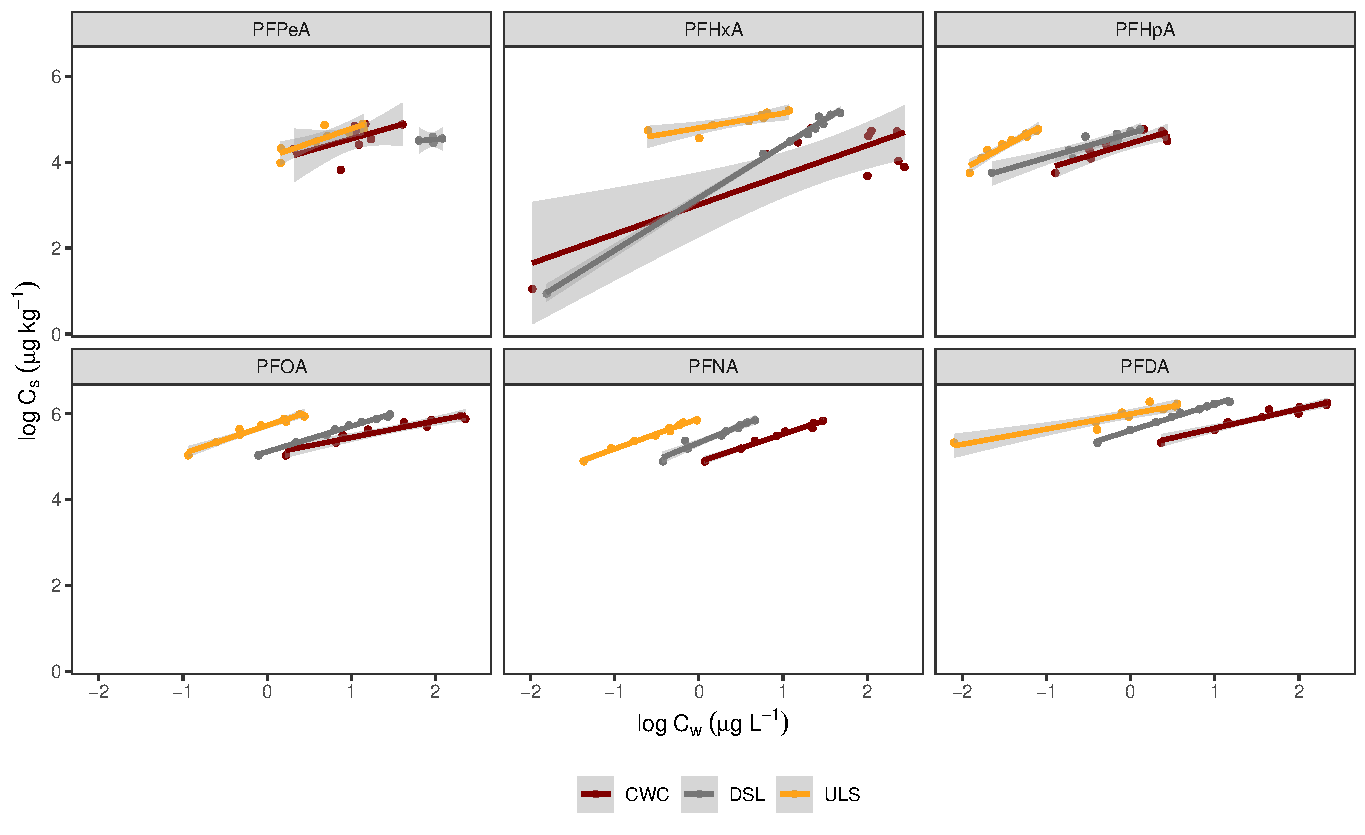
\includegraphics[width=\textwidth]{R/figs/Sorption_isotherms_single_BC.pdf}
    \caption{Freundlich sorption isotherms for PFPeA, PFHxA, PFHpA, PFOA, PFNA and PFDA in batch tests with three different biochars. Lines are obtained by linear regression.}
    \label{fig:sorption_isotherms}
\end{figure}

\begin{table}
\caption{Freundlich sorption parameters of single TC isotherms in CWC, ULS and DSL (n=9). The error is presented as standard error. All $K_F$ data are in units of $\mathrm{(\mu g/kg)/(\mu g/L)^{n_F}}$.}
\centering
\adjustbox{max width=\textwidth}{%
\begin{threeparttable}
\label{tab:summary_stats_single}
\begin{tabular}{lllllllllllll} \toprule
PFCA & \multicolumn{4}{c}{ULS} & \multicolumn{4}{c}{DSL} & \multicolumn{4}{c}{CWC} \\ \cmidrule(l){2-5} \cmidrule(l){6-9} \cmidrule(l){10-13}
 & $\log~K_{F,BC}$ & $n_{F,BC}$ & $r^2$ & $p$ & $\log~K_{F,BC}$ & $n_{F,BC}$ & $r^2$ & $p$ & $\log~K_{F,BC}$ & $n_{F,BC}$ & $r^2$ & $p$ \\ \midrule
PFPeA & 4.10 ± 0.13 & 0.67 ± 0.16 & 0.74 & ** &  &  &  & $>$0.05 &  &  &  & $>$0.05 \\
PFHxA & 4.80 ± 0.06 & 0.34 ± 0.09 & 0.72 & ** & 3.30 ± 0.15 & 1.11 ± 0.11 & 0.93 & *** &  &  & & $>$0.05 \\
PFHpA & 5.98 ± 0.17 & 1.08 ± 0.11 & 0.93 & *** & 4.67 ± 0.06 & 0.57 ± 0.09 & 0.86 & *** & 4.44 ± 0.05 & 0.59 ± 0.11 & 0.80 & ** \\
PFOA & 5.73 ± 0.02 & 0.65 ± 0.05 & 0.95 & *** & 5.12 ± 0.02 & 0.60 ± 0.02 & 0.99 & *** & 5.06 ± 0.08 & 0.39 ± 0.05 & 0.90 & *** \\
PFNA & 5.89 ± 0.02 & 0.71 ± 0.03 & 0.99 & *** & 5.33 ± 0.03 & 0.80 ± 0.07 & 0.94 & *** & 4.88 ± 0.04 & 0.65 ± 0.04 & 0.98 & *** \\
PFDA & 6.00 ± 0.04 & 0.35 ± 0.05 & 0.86 & *** & 5.61 ± 0.02 & 0.61 ± 0.02 & 0.99 & *** & 5.22 ± 0.07 & 0.45 ± 0.04 & 0.94 & *** \\ \bottomrule
\end{tabular}
\begin{tablenotes}
\item Significance codes: *** $<$ 0.001, ** $<$ 0.01
\item Insignificant regressions (p $<$ 0.05) have been removed
\end{tablenotes}
\end{threeparttable}}
\end{table}

\subsection{Effect of PFCA properties}
\begin{landscape}


\begin{figure}[tb]
    \centering
    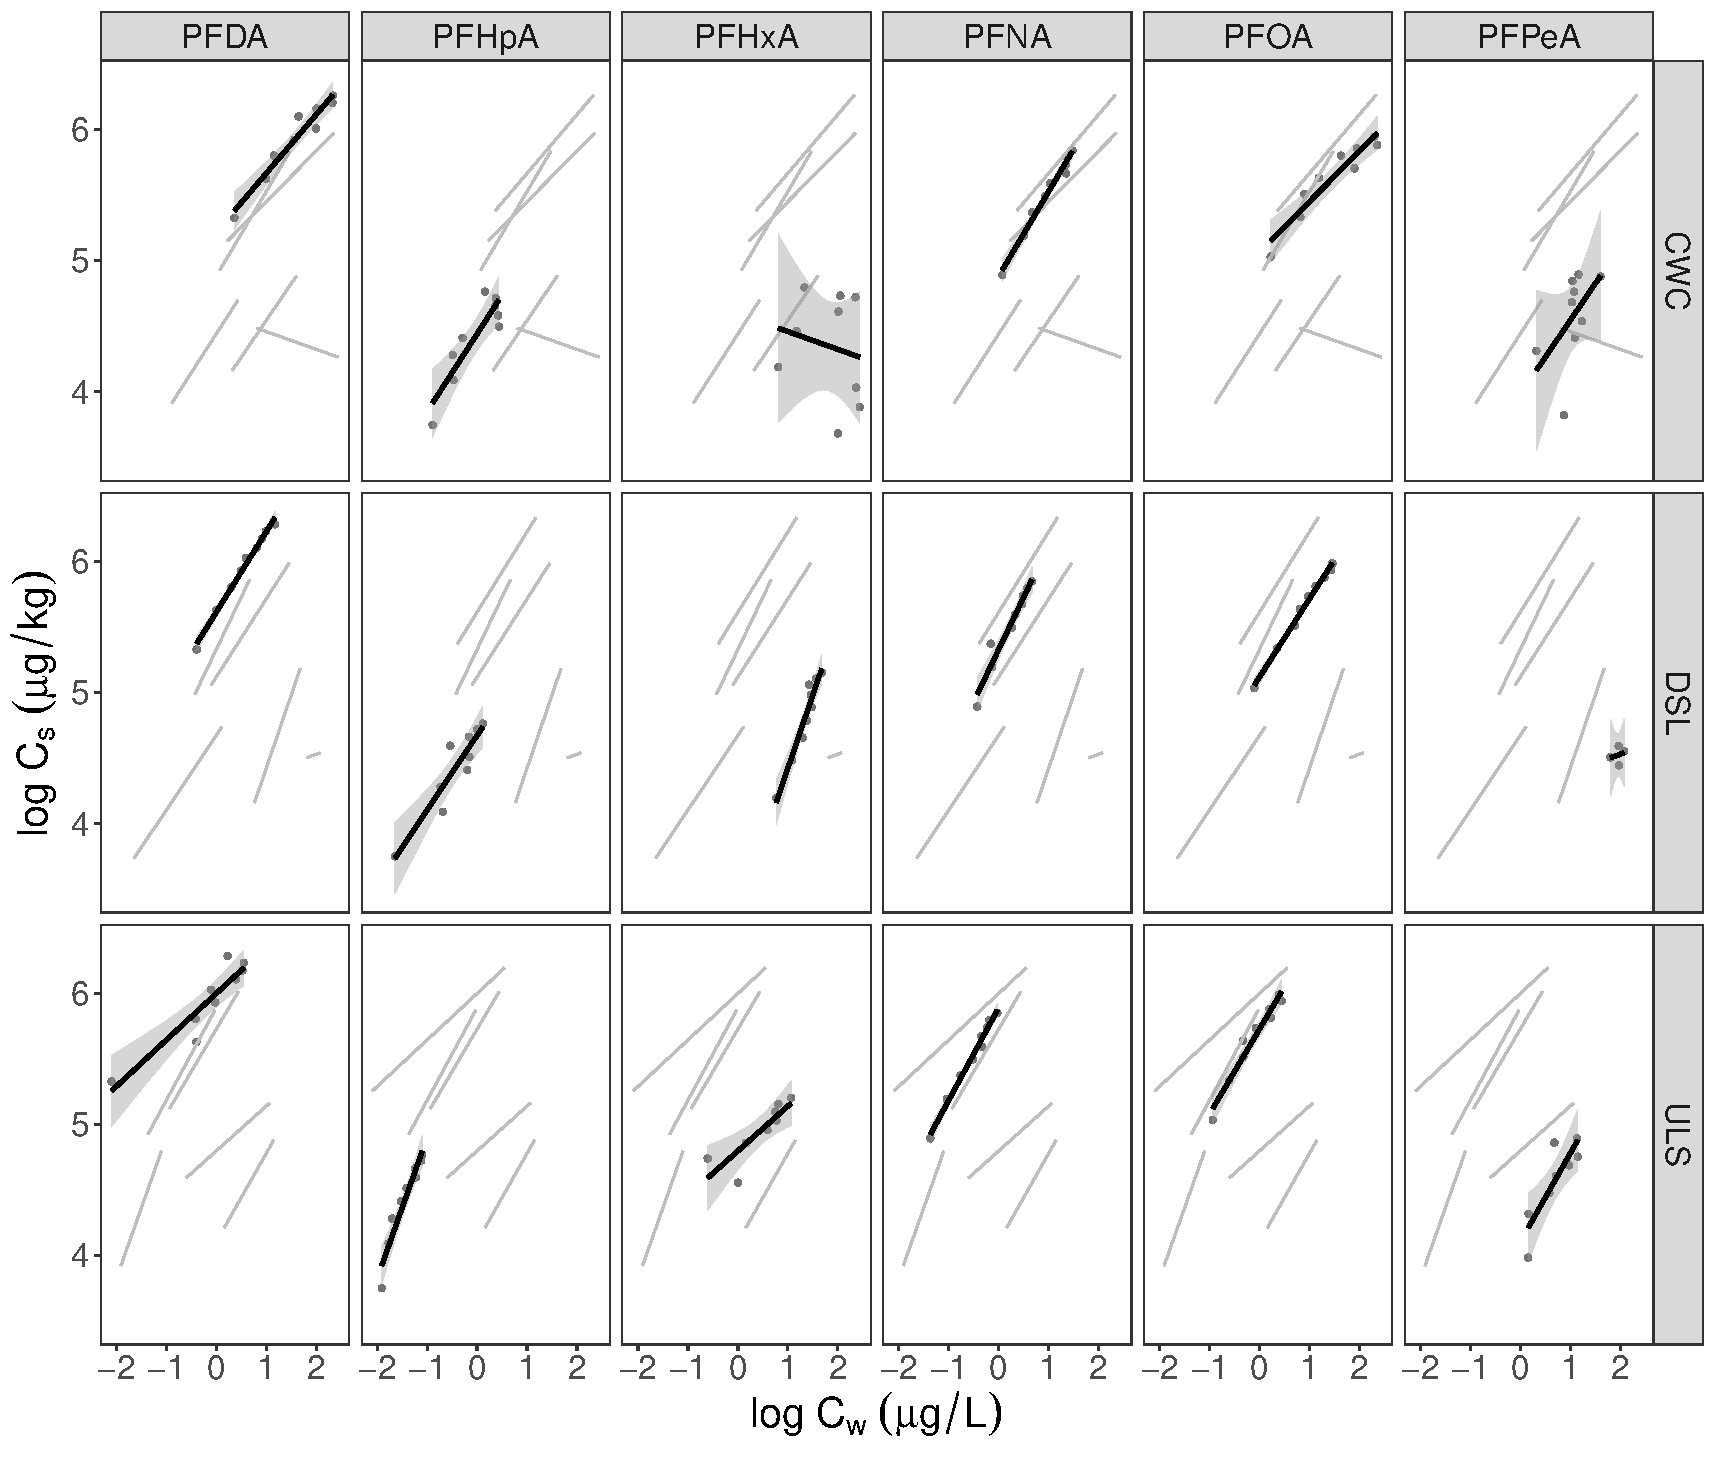
\includegraphics[height=0.8\textheight]{R/figs/BC_facet_isotherm.pdf}
    \caption{Single-compound Freundlich sorption isotherms for PFPeA, PFHxA, PFHpA, PFOA, PFNA and PFDA. Lines are obtained by linear regression. For comparison across chain length, the shaded gray lines are the isotherms from the other compounds with the same sorbent.}
    \label{fig:sorption_isotherms_all}
\end{figure}

\end{landscape} 
\subsubsection{PFCA chain length}
Poor correlations were achieved between the sorbed and aqueous equilibrium concentrations for the short-chain PFCAs (PFPeA, PFHxA, and PFHpA) when sorption isotherms were derived. This can be attributed to poor sorption affinity to biochar.
\cref{fig:sorption_isotherms_all} shows sorption isotherms for the single-compound batch tests for CWC, ULS and DSL. The Freundlich coefficients ($\log~K_F$) for ULS increased in the order: PFPeA (CF4) $<$ PFHxA (CF5) $<$ PFOA (CF7) $<$ PFHpA (CF6) $<$ PFNA (CF8) $<$ PFDA (CF9), ranging from 4.10$\pm$0.13 to 6.00$\pm$0.04, all regressions being significant (p$<$0.01), \cref{tab:summary_stats_single}). The Freundlich coefficients for DSL increased in the order, PFHxA (CF5) $<$ PFPeA (CF4) $<$ PFHpA (CF6) $<$ PFOA (CF7) $<$ PFNA (CF8) $<$ PFDA (CF9), ranging from $\log~K_F$ 3.30$\pm$0.15 to 5.61$\pm$0.02. All regressions were significant (p$<$0.001) except for the PFPeA isotherm which only consisted of four points (SC7-10) because several points that had a higher analyzed filtrate concentrations than what was spiked for SP1-6, had to be omitted due to analytical uncertainty or imprecision/contamination during laboratory work (\cref{fig:sorption_isotherms_all}). The Freundlich coefficients for CWC increased in the order, PFPeA (CF4) $<$ PFHpA (CF6) $<$ PFHxA (CF5) $<$ PFNA (CF8) $<$ PFOA (CF7) $<$ PFDA (CF9), ranging from $\log~K_F$ 3.98$\pm$0.36 to 5.22$\pm$0.07. Regressions were significant (p$<$0.01) except for PFPeA and PFHxA. 

A statistically significant relationship between $\log~K_F$ and CF\textsubscript{2} chain length was found for all three biochars (p$<$0.05) to PFOA, PFNA, and PFDA (\cref{fig:chainlength}). This is in accordance with previous studies \citep{Sorengard2019, higgins2006sorption, ahmed2020per}. There was a difference of 1.2-1.9 $\log~K_F$ units between the longest and the shortest PFCA chain (PFDA and PFPeA). For every CF\textsubscript{2} moiety, hydrophobic interactions between condensed aromatic structures in the biochar matrix increases, contributing to stronger sorption. Several mechanisms can explain why perfluorinated carboxylic acids increase in hydrophobicity with increasing chain length: 1) Due to a high molecular surface of the perfluorinated tail, a high cavity formation energy is needed to dissolve the compounds in water \citep{Arp2006}. For this reason, the compounds tend to be pushed water-solid interfaces, such as a biochar surface. Therefore, dissolution becomes increasingly energetically demanding with increasing chain length \citep{sigmund2022sorption}. 2) The perfluorinated chain is capable of the lowest van der Waals dispersive forces per molecular surface area compared to a hydrocarbon chain \citep{du2014adsorption}. The result is that PFAS has a much weaker attraction than hydrophobic organic compounds to water molecules when in the water cavity. For this reason, PFASs are both oil- and water repellent.  Generally, water cavity formation energy and van der Waals interactions have been considered to be insignificant for sorption of PFAS to solid phases for short-chain molecules (\textless C6) \citep{du2014adsorption}. They are, however, significant for long-chained PFCs (\textgreater C6) \citep{du2014adsorption}.

\begin{figure}[tbh]
    \centering
    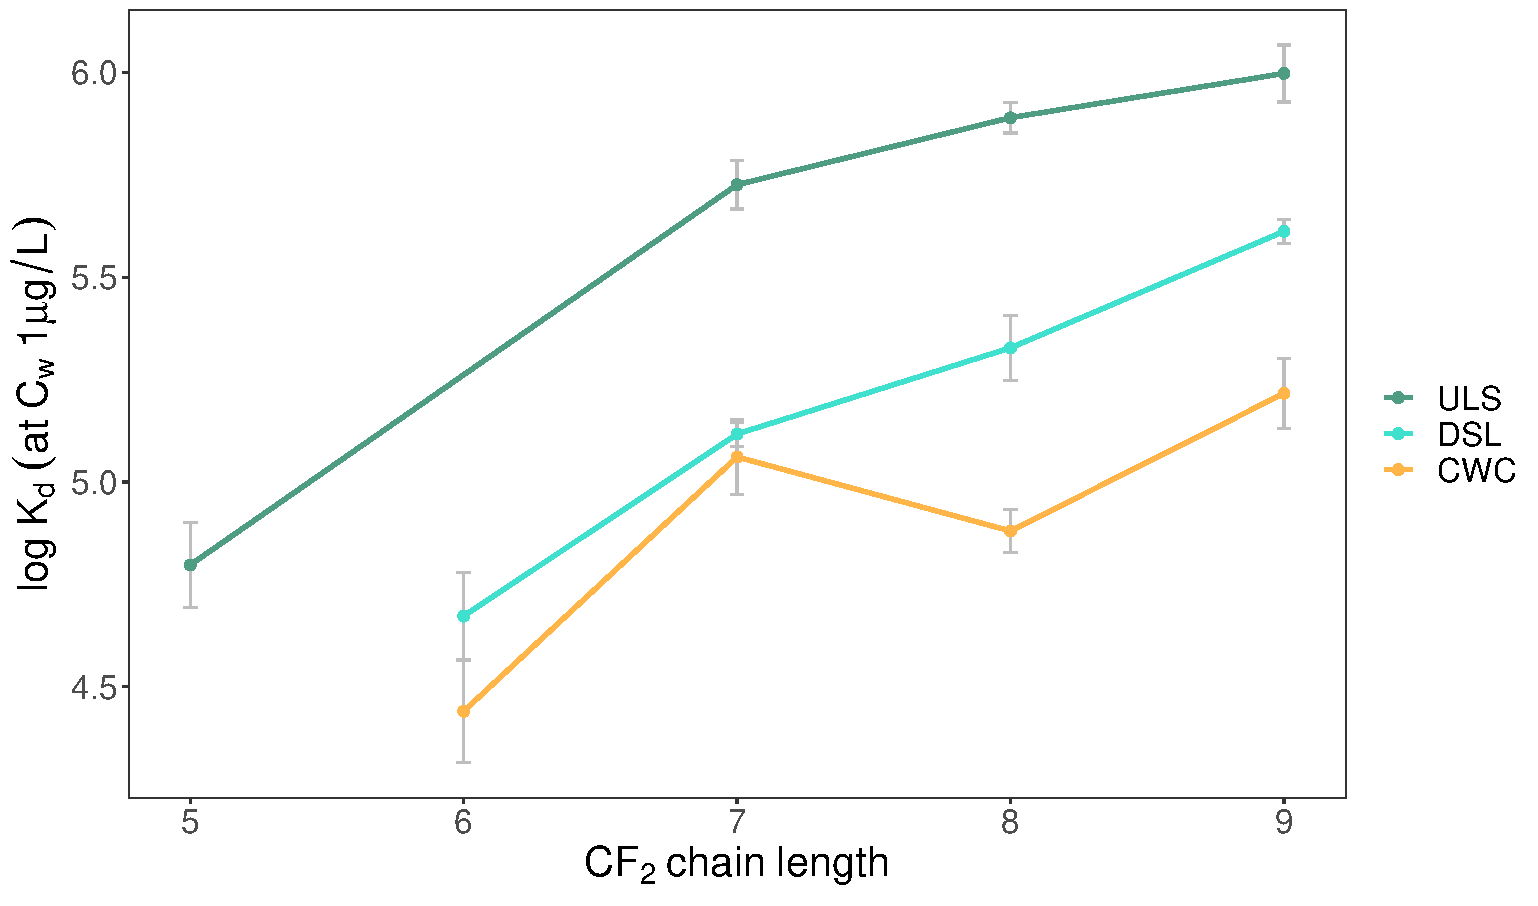
\includegraphics[width=0.7\textwidth]{R/figs/chain_length_Kd1ugL_plot.pdf}
    \caption{Relationship between $\log~K_F$ and chain length. Linear regression coefficients for ULS: $r^2$ = 0.92, $p$ = 0.04, DSL: $r^2$ = 0.98, $p$ = 0.01, CWC: $r^2$ = 0.68, $p$ = 0.17. Error bars are the propagated error of $\log~K_F$ and $n_F$.}
    \label{fig:chainlength}
\end{figure}

\subsubsection{PFAS functional group} 
The charged and polar head of PFCAs gives this compound class unique sorptive properties because the polar head can engage simultaneously in electrostatic bonding with surface functional groups, or bridge cations within the biochar matrix (ash rich in cations) \citep{zhang2013sorption,sigmund2022sorption}. In this study, the highest sorption was seen for ULS and DSL, with the lowest \% carbon (\cref{tab:SAPV}). These results stand in clear contrast to findings in previous literature where it was observed that. However, previous PFAS sorption studies have been conducted on biochar from cleaner, wood-based feedstock \citep{Sormo2021}, activated carbon \citep{zhang2021sorption,Kupryianchyk2016b}, soils and sediments \citep{higgins2006sorption}, and raw sewage sludges \citep{zhang2013sorption}. These studies concluded that the importance of electrostatic interaction to sorption comes secondary to the hydrophobic effect. The main reason for this is that the biochar surface has a net negative charge, and may experience electrostatic repulsion of the negatively charged functional group on PFAS \citep{Ahmad2014}. PFCAs have low $pK_a$s (-1, \citep{goss2008pKa}) due to having strong electron withdrawing fluorine atoms. The PFCAs investigated in this study are negatively charged given the filtrate pH of 7.1-7.4 (\cref{tab:pHcond}). This means that the PFCAs experience electrostatic repulsion from negative sites on the biochar surface, something which accounts for the lowest $K_F$-values for the shorter-chain PFCAs (\cref{tab:summary_stats_single}). This effect is weaker for the longer PFCAs where the hydrophobic effect gets more dominant. 

Electrostatic repulsion is reduced in acid soils where the CEC is reduced, and the biochar surfaces become protonated, and more neutral. This allows for anion- \textpi-bond interaction with biochar \citep{sigmund2022sorption}. The isotherms in \cref{fig:sorption_isotherms_all} show that the measurement points for the short-chain PFCAs (PFPeA, PFHxA and PFHpA) are more scattered, resulting in sorption isotherms with higher standard errors. Sorption is also weaker (lower $\log~K_F$) for these compounds. This can indicate that hydrophobic interactions with the perfluorinated chain are the dominant sorption mechanisms for PFCAs. If electrostatic interactions would be equally important, sorption across chain lengths would be more similar since electrostatic interactions would become increasingly energetically favorable when chain lengths are shorter. However, sorption was shown to increase with chain length onto all three biochars in this study (\cref{fig:chainlength}). A further investigation explaining why the sludge biochars sorb better than CWC is described in the next section.

\cite{zhang2021sorption} found that sorption increased in the order PFBA $<$ PFBS $<$ PFOA $<$ PFOS for granular activated carbon and softwood-derived biochar. The difference between the PFSA and PFCA groups is that PFSAs have one more perfluorinated carbon than PFCAs, which has its terminal carbon bonded as a carboxylate (COO\textsuperscript{-}) instead. If one compares PFHpS to PFOA, which have the same number of $\mathrm{CF_2}$ moieties, the perfluorinated sulfonic acid still sorbs better. Researchers attribute this to: 1) A difference in molecular size because the sulfonate moiety is slightly larger than the carboxylate moiety. This results in a greater cavity formation energy for PFSAs. Hence, in water saturated conditions, the functional group is pushed towards water extremities \citep{yin2022insights,sigmund2022sorption}. In batch shaking experiments, this would be the biochar surfaces or artifacts. 2) Sulfonic acid is a stronger acid than carboxylic acid. This results in a stronger ionic interaction to positive charges of mineral phases in biochar ash \citep{arvaniti2015review}. 

%%%%%%%%%%%%%%%%%%%%%%%%%%%%%%%%%%%%%%%%%%%%%%%%%%%%%%%%%%%%%%%%%%%%%%%%%%%%%%%%%%%%%%%%%%%%%%%%%%%%%%%%%%%%%%%%%%%%%%%%%%%%%%%%%%%%%%%%%%%%%%%%%%%%%%%%%%%%%%%%%%%%%%%%%%%%%%%%%%%%%%%%%%%%%%%%%%%%%%%%%%%%%%%%%%%%%%%%%%%%%%%%%%%%%%%%%%%%%%%%%%%%%%%%%%%%%%%%%%%%%%%%%%%%%%%%%%%%%%%%%%%%%%%%%%%%%%%%%%%%%%%%%%%%%%%%%%%%%%%%%%%%%%%%%%%%%%%%%%%%%%%%%%%%%%%%%%%%%%%%%%%%%%%%%%%%%%%%%%%%%%%%%%%%%%%%%%%%%%%%%%%%%%%%%%%%%%%%%%%%%%%%%%%%%%%%%%%%%%%%%%%%%%%%%%%%%%%%%%%%%%%%%%%%%%%%%%%%%%%%%%%%%%%%%%%%%%%%%%%%%%%%%%%%%%%%%%%%%%%%%%%%%%%%%%%%%%%%%%%%%%%%

\section{The effect of biochar properties on sorption}
This section relates the distribution coefficients derived for ULS, DSL and CWC biochars to the following BC characteristics: main elements (C, H, O, N), trace elements (Ca and Fe), surface area (SA), and pore volume (PV) in an attempt to gain insight into possible sorption mechanisms. In the comparison between sorbent properties and sorption coefficients for each biochar feedstock, PFOA, PFNA and PFDA have been used because they exhibited the best sorption isotherms. The Freundlich coefficients ($\log~K_F$) have been normalized to 1 $\mu g~L^{-1}$ which is used as the distribution coefficient ($K_d$) in this discussion. Conducting multivariate analyses between biochar $K_d$ and the different supporting parameters for the biochar samples were desired but not statistically valid due to no degrees of freedom with only 3 samples. Therefore, the discussion on the effects of biochar properties on sorption will be limited to discerning trends with SA, PV, C, Ca and Fe. 

\subsection{Surface area and pore volume}

\begin{table}
\centering
\caption{Surface area (SA), pore volume (PV), elemental content (C, O, H, N) and ratios for the biochars produced for the batch tests.}
\adjustbox{max width=\textwidth}{
\label{tab:SAPV}
\begin{tabular}{llrrrrrrlllllll}
\toprule
Biochar & \multicolumn{4}{l}{N\textsubscript{2} sorption} & \multicolumn{3}{l}{CO\textsubscript{2} sorption} & \multicolumn{4}{c}{Elemental content} & \multicolumn{3}{c}{Elemental ratio} \\
sorbent & \multicolumn{4}{l}{(pores \textgreater 1.5 nm)} & \multicolumn{3}{l}{(pores 0.4-1.5 nm)} & & & & & & \\ \cmidrule(l){2-5} \cmidrule(l){6-8} \cmidrule(l){9-12} \cmidrule(l){13-15} 
& BET SA  & BJH PV & log SA/PV & log SA/PV/C & DFT SA & DFT PV & log SA/PV & C & O & H & N & O/C & H/C & N/C \\
& ($\mathrm{m^2~g^{-1}}$) & (cm\textsuperscript{3} g\textsuperscript{-1}) & ($\mathrm{m^2 cm^{-3}}$) & ($\mathrm{m^2 cm^{-3} g^{-1}}$)& ($\mathrm{m^2~g^{-1}}$) & (cm\textsuperscript{3} g\textsuperscript{-1}) & ($\mathrm{m^2 cm^{-3}}$) & (\%) & (\%) & (\%) & (\%) & & & \\ \midrule
CWC & 323 & 0.017 & 4.28 & 2.32 & 683 & 0.186 & 3.54 & 91.4 & 5.50 & 1.01 & 0.69 & 0.06 & 0.01 & 0.008       \\
ULS & 128 & 0.126 & 3.01 & 1.54 & 165 & 0.047 & 3.57 & 29.6 & 57.1 & 1.24 & 1.13 & 1.9  & 0.04 & 0.04        \\
DSL & 110 & 0.111 & 3.00 & 1.87 & 87  & 0.027 & 3.51 & 13.5 & 61.4 & 1.05 & 0.82 & 4.6  & 0.08 & 0.06       \\ \bottomrule
\end{tabular}}
\end{table}

\subsubsection{Pore size distribution between 0.4-1.5 nm}
\cref{tab:SAPV} shows the total surface area (SA, m\textsuperscript{2}/g) and pore volume (PV, cm\textsuperscript{3}/g) for the three biochars used in the sorption experiments in this study. SA of CWC biochar (683 m\textsuperscript{2} g\textsuperscript{-1}) was $\sim$six times higher than that of ULS and DSL biochars (165 and 87  m\textsuperscript{2} g\textsuperscript{-1}, respectively), and PV also reflected the same order. Previous research has postulated that large internal surface areas and pore volumes are desirable for strong sorption of organic contaminants because they increase the fraction of active sorption sites \citep{ahmed2020per,Hale2016}. The high SA and PV of CWC suggest that this biochar has the highest fraction of active sites compared to ULS and DSL within the micropore range ($\le$ 2 nm). Pore size distribution (PSD) in terms of SA and PV of pores available for CO\textsubscript{2} adsorption (0.4-1.5 nm) is shown in \cref{fig:PZD_small}, where it becomes becomes evident that nearly 80\% of the SA and 60\% of the PV of CWC are located in pores smaller than 0.6 nm. These are referred to as ultra micropores \citep{bardestani2019experimental}. To find out whether PFCAs can be accommodated in these ultra micropores, \cref{tab:molecsize} lists effective cross-sectional diameter ($D_{eff}$) and maximum diameter ($D_{max}$) of each PFCA (the definitions of $D_{eff}$ and $D_{max}$ are illustrated in \cref{fig:molecularSize}). PFCAs C5-C10 range from 0.45-0.72 nm ($D_{eff}$) to 0.96-1.54 nm ($D_{max}$). Since the respective perfluorinated chains are too large and rigid to enter, most pores ($<$ 0.6 nm)turned out to be inaccessible to the PFCA molecules \citep{yu2009sorption}. Additionally, pores that are too small make it difficult for the compounds to adjust their shape to the pore walls in order to be able to come close enough to sorb to the pore wall surface. For this reason, they may get stuck in a cross-sectional position that blocks the pores for diffusion of new sorbates. 

Maximum sorption is achieved when the molecular dimensions of PFAS match the pore size and shape of the sorbent \citep{Hale2016}. Since the PSD within the CO\textsubscript{2}-range is dominated by ultra micropores, sorption of PFPeA, PFHxA, and PFHpA is only possible if the congeners enter the pores at the exact right angle. PFOA, PFNA, and PFDA will experience size exclusion because the molecular size is too large in any direction (\cref{tab:molecsize}). In addition, these pores are easily blocked. This means that sorption of PFAS in the CO\textsubscript{2}-range is insignificant and cannot explain the differences in the $\log~K_F$ obtained for the biochar feedstocks, especially since strongest sorption was measured for long-chain PFCAs.

The surface area to pore volume ratio (SA/PV) can be used to more accurately represent available sorption sites, where a lower ratio indicates higher porosity \citep{presser2011SAPV}. Since PV increases by increasing pore diameter (\cref{fig:PZD_small}), the relative increase in PV will be higher than the relative increase in SA. This means that the SA/PV ratio is expected to decrease more rapidly for biochar with higher pore volumes. This expectation is confirmed in \cref{fig:PZD_small} where the SA/PV ratios for ULS and DSL are nearly equivalent to CWC, despite the fact that SA and PV are significantly different from CWC taken separately. This is reflected in the cumulative SA/PV ratios (\cref{tab:SAPV}) which are similar: 3 674, 3 502, and 3 206 m\textsuperscript{2} cm\textsuperscript{-3} for CWC, ULS, and DSL respectively. This means that despite CWC being more numerous in micropores than ULS and DSL, its porosity is similar, and is predominantly allocated within the ultra micropore fraction.

\begin{figure}[htb]
    \centering
    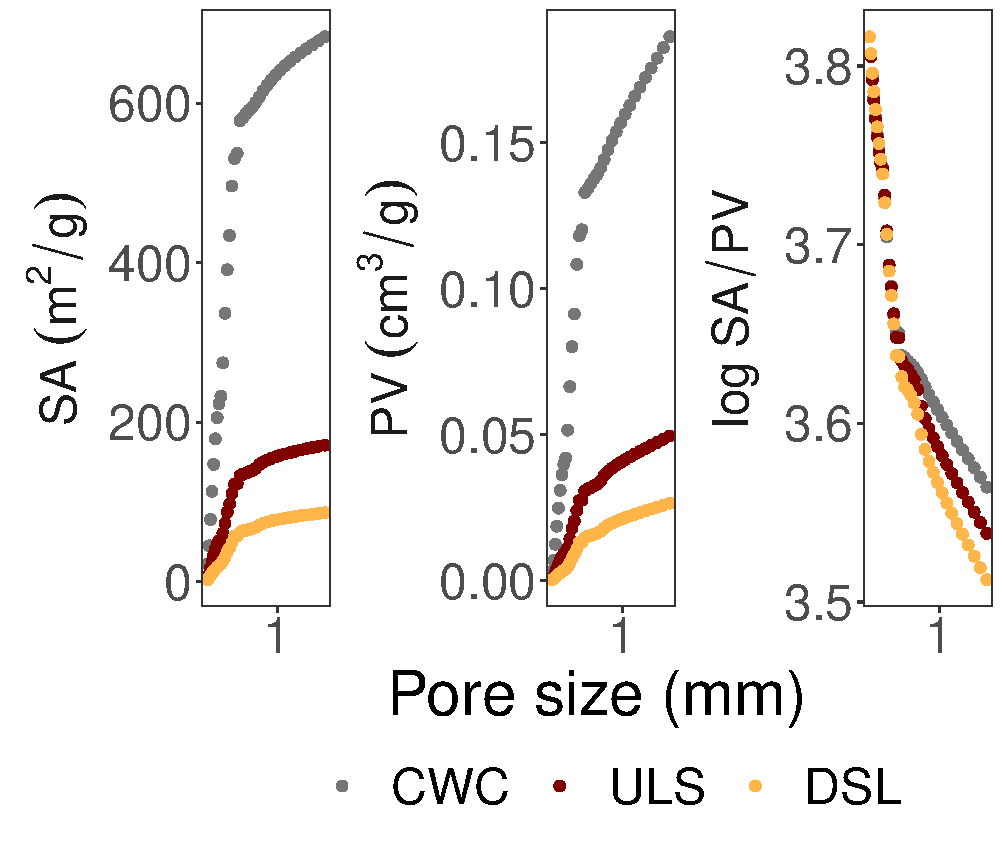
\includegraphics[width=\textwidth]{R/figs/PZD_SAPV_C_small_plot.pdf}
    \caption{Cumulative pore size distribution for pores 0.4-1.5 nm using DFT.}
    \label{fig:PZD_small}
\end{figure}

\begin{table}
\caption{Effective cross-sectional diameter ($D_{eff}$) and maximum diameter ($D_{max}$) of TCs interpolated and extrapolated by linear regression from calculations performed by \cite{inoue2012size} on PFOA and other PFCAs with chain lengths 11-18.}
\centering
\begin{threeparttable}
\label{tab:molecsize}
\begin{tabular}{lcrr}
\toprule
Compound & Chain & $D_{eff}$ & $D_{max}$ \\ 
& length & (nm) & (nm) \\ \midrule
PFPeA & 5  & 0.45  & 0.96  \\
PFHxA & 6  & 0.50  & 1.08  \\
PFHpA & 7  & 0.56  & 1.19  \\
PFOA\textsuperscript{*} & 8 & 0.61 & 1.36 \\
PFNA & 9 & 0.67 & 1.42  \\
PFDA & 10 & 0.72 & 1.54  \\ \bottomrule                                    
\end{tabular}
\begin{tablenotes}
\item \textsuperscript{*} Value from \cite{inoue2012size}
\end{tablenotes}
\end{threeparttable}
\end{table}

\begin{figure}
    \centering
    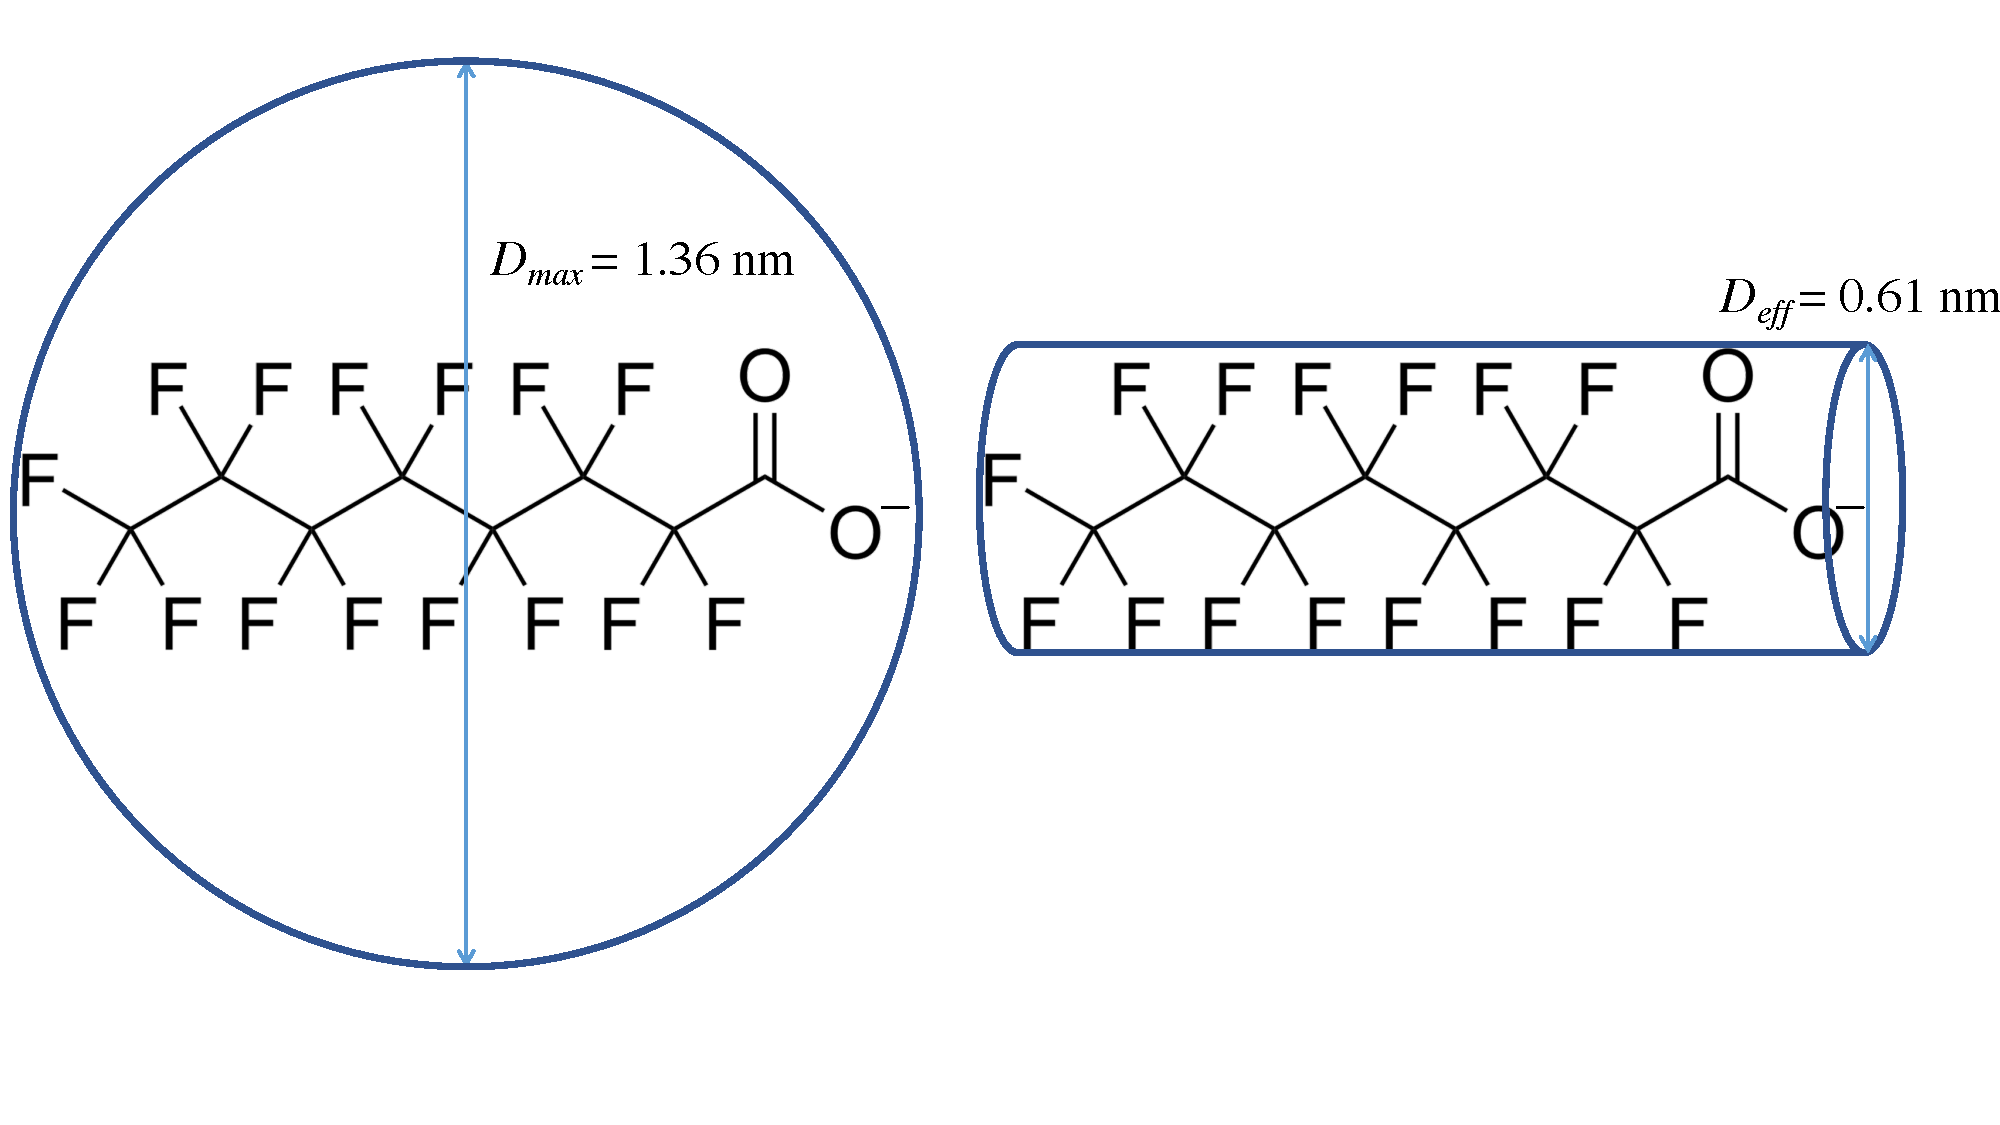
\includegraphics[width=0.8\textwidth, trim={0 2cm 0 0},clip]{Diagrams/Molecular_size.pdf}
    \caption{Definition of effective cross-sectional diameter ($D_{eff}$) and maximum diameter ($D_{max}$) shown for PFOA.}
    \label{fig:molecularSize}
\end{figure}

\subsubsection{Pore size distribution for pores $>$1.5 nm}
Similar to the trend for small pores, CWC also had the largest cumulative SA but the lowest PV for pores $>$1.5 nm (323 m\textsuperscript{2} g\textsuperscript{-1} versus 110 and 128 m\textsuperscript{2} g\textsuperscript{-1} for DSL and ULS, respectively). \cref{fig:PZD_large}a shows that the highest proportion of SA is allocated to pores between 1.5-3 nm for CWC and 1.5-5 nm for ULS and DSL. Cumulative PV is highest for ULS (0.126 cm\textsuperscript{3} g\textsuperscript{-1}), where PV for CWC was one order of magnitude lower (0.017 cm\textsuperscript{3} g\textsuperscript{-1}). Furthermore, the development of PV with pore diameter in \cref{fig:PZD_large}b shows a clear distinction between CWC and the two sewage sludge biochars. CWC has most of its PV in pores $<$3 nm, whereas PV for ULS and DSL steadily increase up to the maximum pore size of 35 nm. This difference becomes important for the SA/PV ratio seen in \cref{fig:PZD_large}c. Here, ULS and DSL have low and equivalent cumulative $\log~SA/PV$ ratios of 2.8 compared to the higher ratio of 3.2 for CWC (\cref{tab:SAPV}). Previous studies have consistently concluded that a large internal surface area and pore volume of adsorbents are the two most important parameters for achieving high sorption capacity of PFAS \citep{du2014adsorption,Sormo2021,Hale2016,ahmed2020per}. Similarly, the results of this study provide clear indications that a low SA/PV ratio can be considered a proxy for good PFAS sorption. The most plausible explanation for why CWC is the weakest sorbent among the three samples in this study is that CWC consists almost exclusively of micropores, whereas ULS and DSL also have pores in the mesopore range (2-50 nm). The shift observed by comparing SA and PV together demonstrates the importance of considering both pore size \textit{and} surface area when evaluating available sorption sites on biochar.

Since ULS and DSL had nearly equivalent SA/PV ratios, an additional parameter is needed to explain why ULS is a better sorbent than DSL (\cref{fig:PZD_large}c). Apart from SA and PV, carbon content has, in previous literature, been a good predictor of sorption affinity to PFAS \citep{Hale2016,Cornelissen2005}. ULS contains 29.6 \% carbon whereas DSL contains 13.5 \%.  

Similar to \cref{fig:PZD_large}, \cref{fig:Kd_SAPV_C} shows the relationship between each of carbon content ($\log~C$), $\log~SA/PV$ and $\log~SA/PV/C$, now as a function of $\log~K_d$ (normalized to 1 $\mu g~L^{-1}$). This figure shows that a linear relationship exists between $\log~K_d$ and $\log~SA/PV/C$, and that no such relationship is present for carbon content and the SA/PV ratio individually. This means that high porosity and sufficiently large pores are the two most important parameters that regulate high sorption capacity, and that the pore wall composition further contributes to enhanced sorption. 

\begin{figure}[htb]
    \centering
    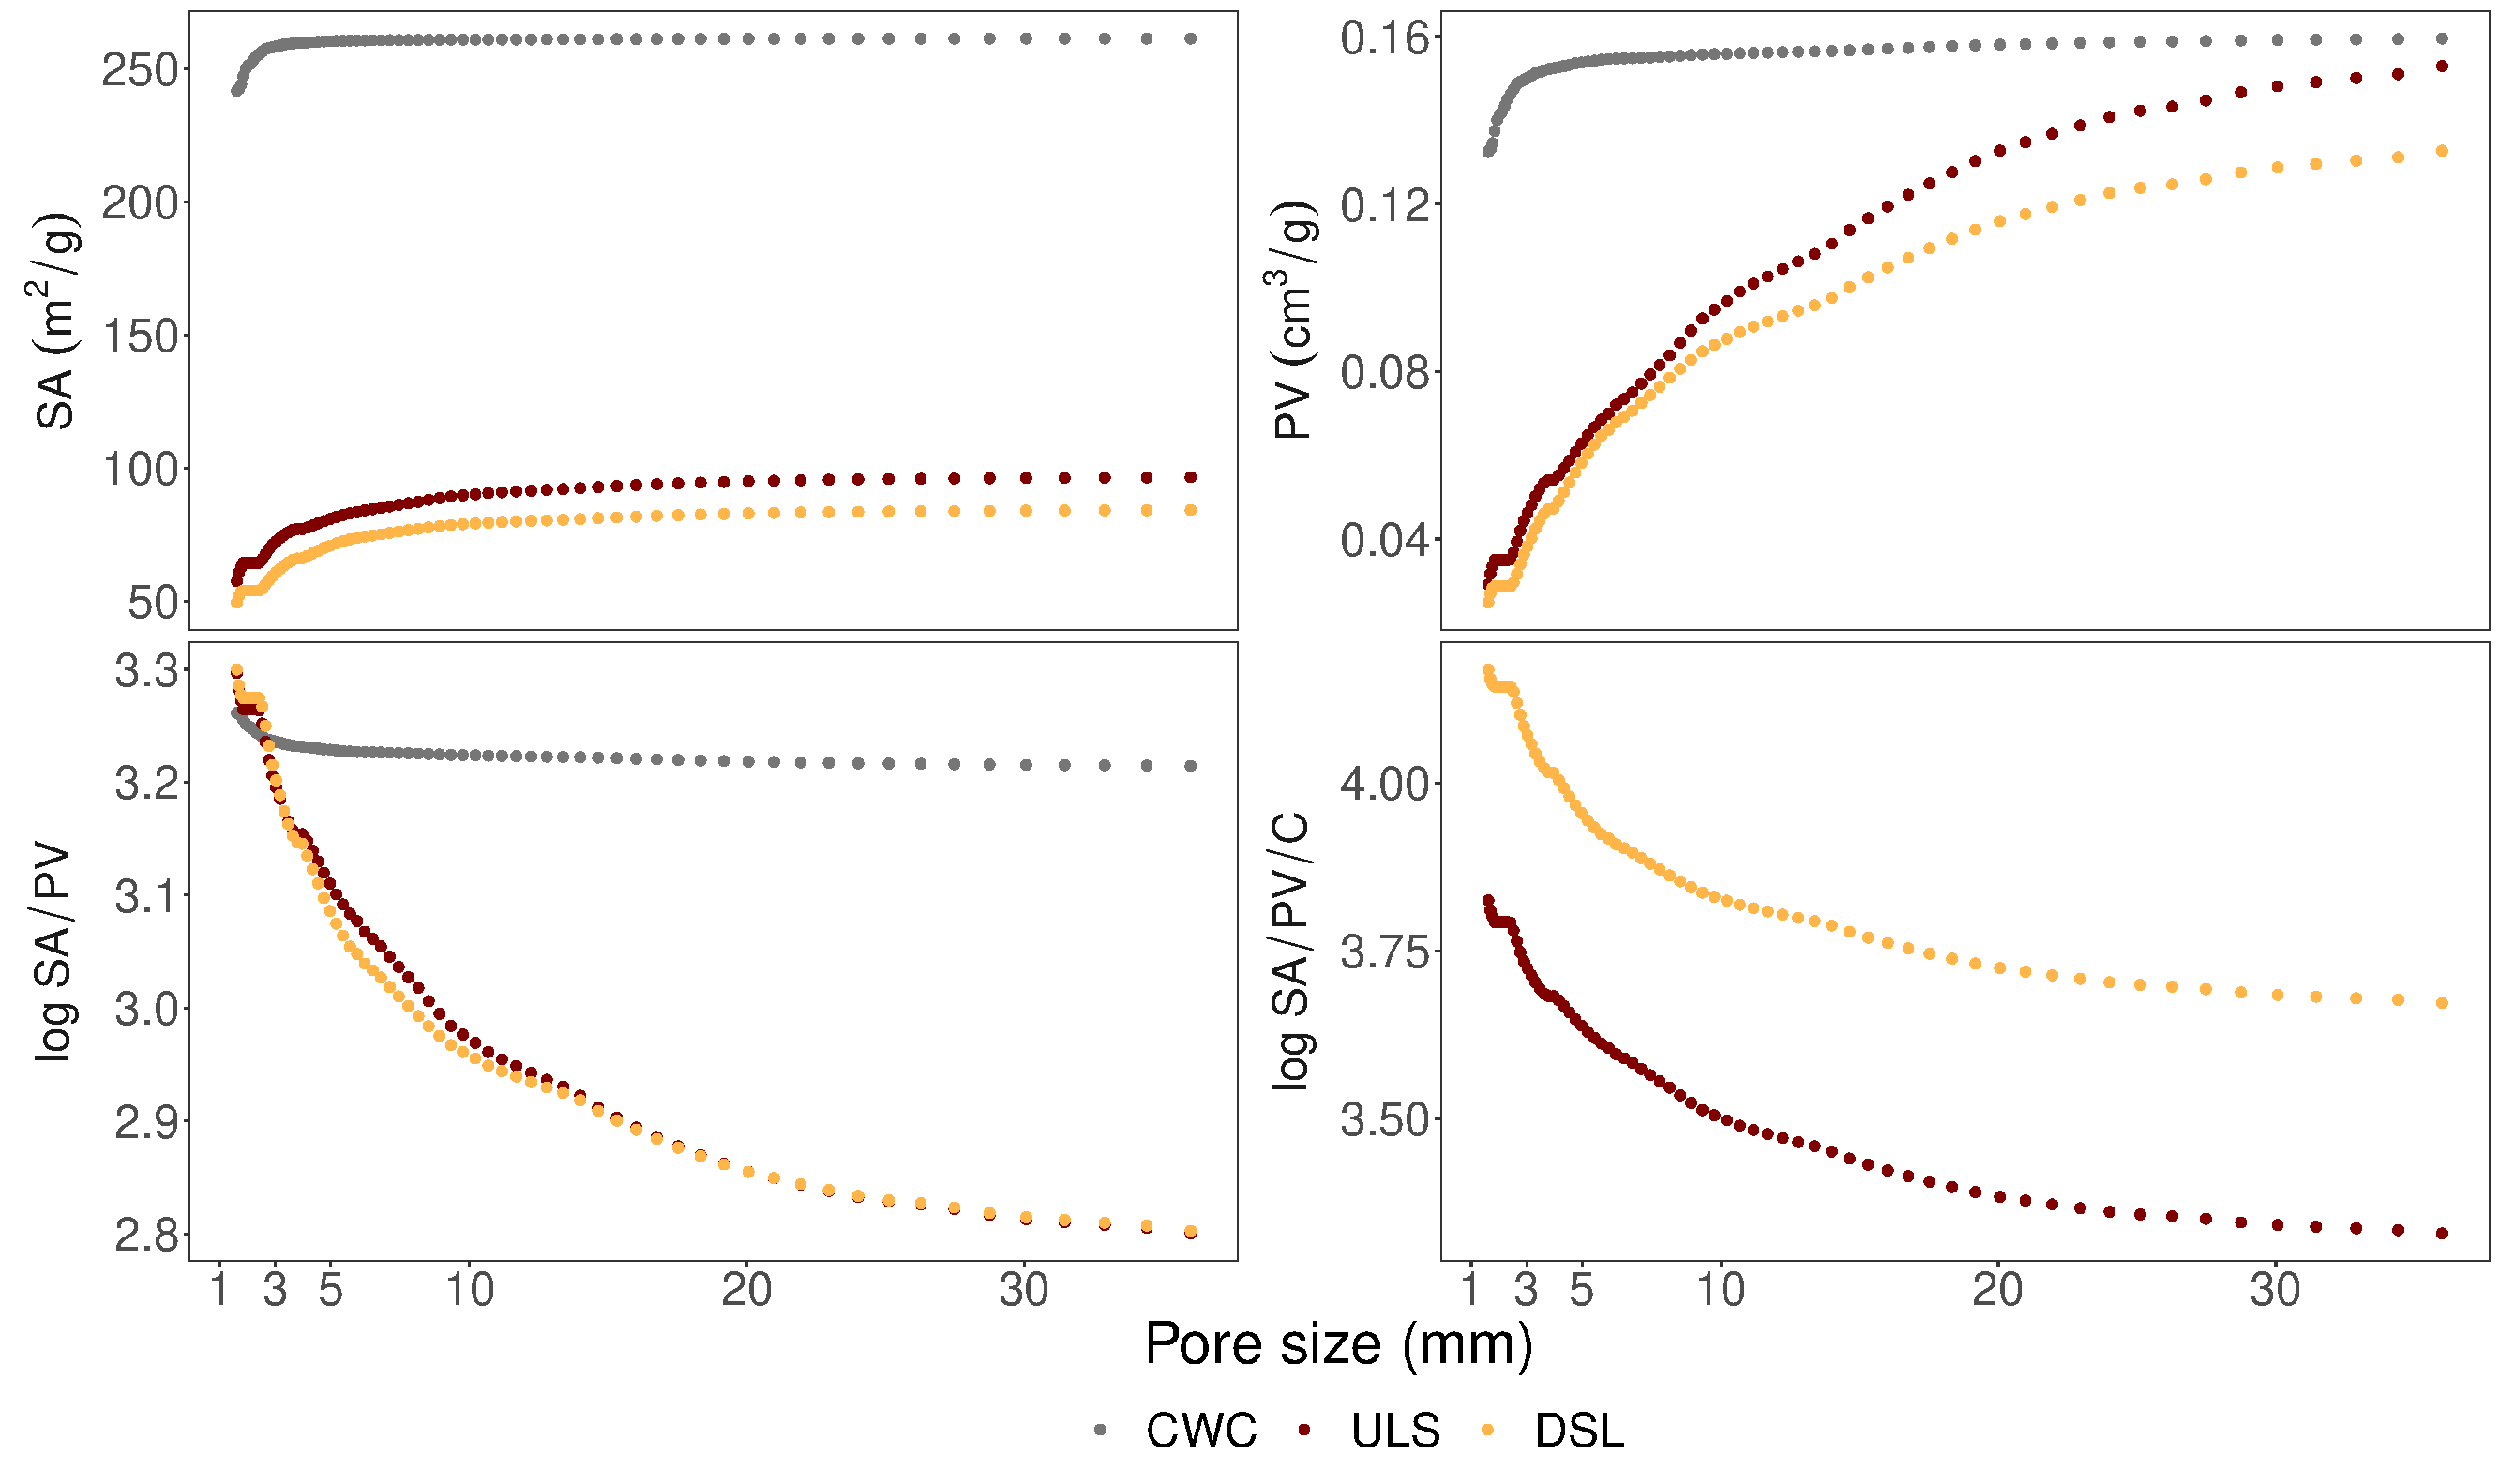
\includegraphics[width=\textwidth]{R/figs/PZD_SAPV_C_large.pdf}
    \caption{Cumulative pore size distribution for pores $>$ 1.5 nm using DFT theory. (a) Surface area, (b) pore volume, (c) SA/PV ratio for pores $>$1.5 nm normalized to carbon content (g C/g BC). (d) A lower SA/PV/C ratio indicates a higher degree of C in the pore wall matrix.}
    \label{fig:PZD_large}
\end{figure}

\subsection{Biochar surface chemistry}
The total composition of elements other than carbon may provide further insight into how the pore walls of CWC, ULS and DSL differ from one another, and how these differences influence sorption. The proportion of elements other than C, O, H and N contained in the biochar matrices was significantly lower for the clean wood biochar (1.4 \%) compared to sludge biochars (10.9 and 23.2 \%). Total elemental composition of the biochars is given in \cref{appSec:elements}. Surface hydrophobicity and degree of carbonization can be described by O/C, H/C, and N/C ratios \citep{chun2004compositions}. As reported previously, the O/C ratio of CWC (0.06) is within the same range as non-activated biochars pyrolyzed at 700\textdegree C \citep{LehmannAndJoseph2015, chun2004compositions,kupryianchyk2016biochar}. By contrast, the high oxygen content of DSL and ULS (61.4 and 57.1 \% respectively) results in increased O/C ratios of 4.6 and 1.9 respectively (\cref{tab:SAPV}). The difference between the O/C ratio \textless 1 for CWC compared to ratios \textgreater 1 for ULS and DSL indicate a significantly different degree of carbonization between the two feedstock types. At the same time, H/C ratios for all three biochar feedstocks are similar, and within the same range reported in previous literature \citep{chun2004compositions,kupryianchyk2016biochar}. 

A higher O/C and N/C ratio---indicative of more polar functional groups (hydroxyl, carbonyl, metal-containing groups, amines and amides)---has proven to be beneficial for PFAS sorption \citep{du2014adsorption}. Researchers suggest several mechanisms related to surface polar groups that may contribute to enhanced sorption. First, basic functional groups such as amines have high $pK_a$s and are protonated at environmentally relevant pH providing anion exchange capacity and electrostatic attraction to the carboxylic acid heads \citep{deng2010removal}. N/C ratios for ULS and DSL are one order of magnitude higher than CWC. A high nitrogen/carbon (N/C) ratio can be indicative of more amine groups in the periphery of the condensed carbon structure. The positive charge on the nitrogen-containing functional groups can interact electrostatically with the PFCA carboxylate group. In addtion, it is possible that they also engage in weak non-specific electrostatic interactions with the negative dipole of the CF-chain \citep{xiao2011effects}. The latter mechanism could explain the positive chain-length dependency on sorption seen for the sewage sludge biochars (\cref{fig:chainlength}) in addition to the low SA/PV/C ratio discussed in the previous section. Sewage sludge contains a homogeneous mixture of proteins and inorganic nutrients that will denaturate in some form during thermal treatment. To the author's knowledge, no data exists on how speciation of nitrogen changes during pyrolysis. Even though a higher N/C ratio is only an indication for nitrogen functional groups, the presence of amines is likely. Second, since sludge chars contain more ash than CWC, divalent cations such as Ca\textsuperscript{2+} and Mg\textsuperscript{2+} will bind to basic sites on the biochar surface and form divalent cation bridges to PFAS \citep{higgins2006sorption}. This is further discussed in \cref{sec:inorganic}. Although sorption \textit{capacity} has not been measured directly, the above-mentioned mechanisms for PFAS interaction with charged and polar functional groups may be contributors to the higher sorption found for the more heterogeneous, mineral-rich matrices of the sewage sludge biochars. 

\subsubsection{Iron speciation}
Due to the lack of corresponding reference compounds for some of the EXAFS signals, no satisfying fit was obtained for the iron species present in the sewage sludge biochar samples. This information indicates that iron is not only present as iron oxides. The Fe K-edge XANES spectra (\cref{appFig:valence}) and EXAFS spectra (\cref{appFig:Fe_species}) show that DSL and ULS are similar in valence and speciation. They mainly consist of reduced forms of Fe (Fe(II)), and DLS is slightly more reduced than ULS. Total Fe concentration is especially high for DSL (180 mg/kg, \cref{tab:BC_mainElements}), making up as much as 18\% of its matrix (3.3\% and 0.01\% for ULS and CWC respectively). The Fe concentration will therefore significantly affect surface morphology of DSL. PFAS has been shown to form inner-sphere complexes via covalent metal-ligand bonds (Fe-carboxylate) by means of the following reaction \citep{du2014adsorption}:

\begin{equation}
    \mathrm{\equiv Fe-OH_2^+ ~ + ~ CF_3(CF_2)_nCOO^- \rightarrow ~ \equiv Fe-OOC(CF_2)_nCF_3 ~+~ H_2O}
\end{equation}

where the triple bond represents chelation of Fe to the biochar matrix. Point of zero charge (pzc) for Fe(oxyhydr)oxides, such as ferrihydrite and goethite, are around 7, similar to the solution pH measured for the water-biochar systems (see \cref{sec:inorganic}). The iron species are expected to be neutral for the systems analyzed and will likely not be one of the dominating sorption mechanisms for PFCA. 

\begin{table}
\centering
\caption{Mean pH and conductivity (\textmu S cm\textsuperscript{-1}) measurements for the different batch test systems (n=3). BC/S/L is the biochar:soil:liquid ratio.}
\label{tab:pHcond}
\begin{tabular}{lccccc}
\toprule
 & \multicolumn{2}{c}{pH} & \multicolumn{2}{c}{Conductivity} & \\ \cmidrule(l){2-3} \cmidrule(l){4-5}
 & mean & std. error & mean & std. error & BC/S/L\\ 
\midrule
ULS & 7.10 & 0.03 & 45.7 & 1.8 & 1/0/500\\
DSL & 7.31 & 0.01 & 40.9 & 0.6 & 1/0/500\\
CWC & 7.36 & 0.04 & 46.5 & 0.4 & 1/0/500\\
ULS+S & 7.18 & 0.01 & 34.9 & 0.2 & 1/50/500\\
DSL+S & 7.14 & 0.003 & 35.7 & 0.9 & 1/50/500\\
CWC+S & 7.09 & 0.03 & 44.9 & 0.9 & 1/50/500\\
S & 7.08 & 0.03 & 23.3 & 0.9 & 0/1/10\\
\bottomrule
\end{tabular}
\end{table}

\begin{figure}[htb]
    \centering
    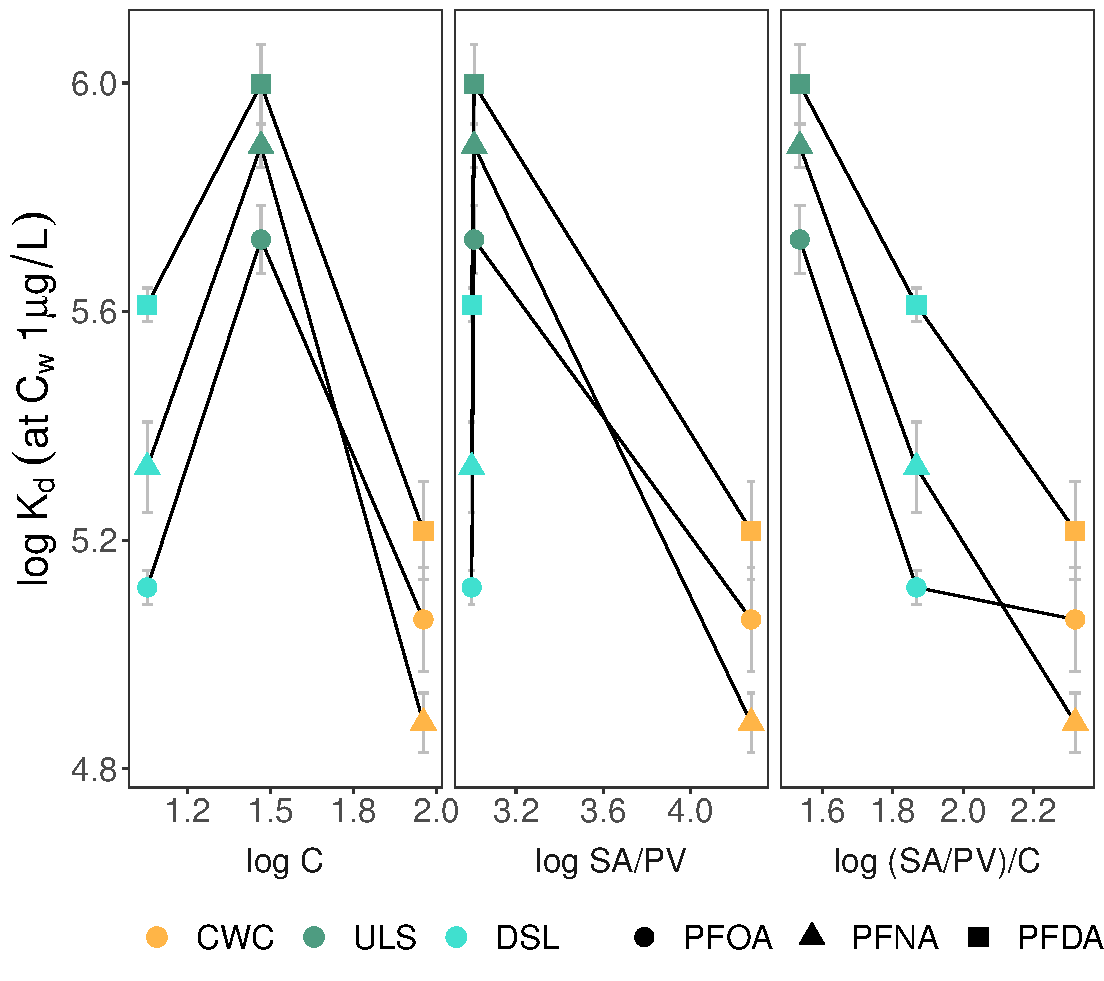
\includegraphics[width=0.8\textwidth]{R/figs/SAPV_C_Kd1ugL_plot.pdf}
    \caption{The correlation of $\log~K_d$ vs. (a) log C (b) log SA/PV (c) log (SA/PV)/C using BET for SA and BJH for PV by biomass feedstock. The points are discrete measurements, and the lines have been added to indicate trends. Error bars are the propagated standard error of $\log~K_F$ and $n$.}
    \label{fig:Kd_SAPV_C}
\end{figure}

\subsection{Effect of solution chemistry}\label{sec:inorganic}

Since dissolved ions were not analyzed, an assumption based on the total element composition of the biochar is made for the discussion of potential roles of inorganic ions for PFAS sorption. Consistent with expectations, the sludge chars have the highest mineral content overall. Coexisting inorganic cations and anions complicate the sorption behavior of PFCAs, where several mechanisms are involved in changing both solution and biochar surface morphology \citep{du2014adsorption}. The presence of ions can both enhance or suppress sorption through mechanisms such as surface-charge neutralization and divalent cation bridging \citep{du2014adsorption}.

pH varied little across sample types with an average pH of 7.18 $\pm$ 0.02 (complete pH and conductivity in \cref{appSec:misclab}). Since variance was low, pH and conductivity are only used to discuss expected surface charges. Adsorption capacity of PFAS has been shown to increase at lower pH because the biochar surface is usually negatively charged at neutral pH \citep{zhang2013sorption}. However, high contents of divalent cations such as Ca\textsuperscript{2+} and Mg\textsuperscript{2+} and iron (Fe) species in the sewage sludge biochars can enhance sorption through cation-bridging between a negatively charged biochar surface and a carboxylate of the PFCA \citep{sigmund2022sorption}. As discussed in \cref{sec:physchem}, this interaction is stronger than the hydrophobic interaction between the CF-chain and the biochar surface.

Composition of earth alkalis is similar for ULS and DSL, whereas the concentration of Ca and Mg for CWC is, respectively, one and two orders of magnitude lower(\cref{tab:BC_mainElements}. Bridging has been shown to be an important sorption mechanism in, for example, sediments, mineral materials, and black carbon \citep{higgins2006sorption}. Apart from bridging between the BC surface and PFAS functional groups, divalent ions can be bridges between individual PFAS molecules. This creates an even more hydrophobic complex that can sorb more strongly to biochar. Both Ca\textsuperscript{2+} and Mg\textsuperscript{2+} have been reported to engage in the chaining of perfluorinated carboxylic acids \citep{wang2011}.

%PZC data? (A high point of zero charge (PZC) therefore increases the adsorption capacity because the surface functional groups are more likely to be protonated).

\begin{table}
\centering
\caption{Composition of a selection of elements in the biochar samples in g/kg.}
\label{tab:BC_mainElements}
\begin{tabular}{lrrrrrrrr} \toprule
 & Ca & Fe & K & Mg & Na & P & S & Si \\ \midrule
CWC & 8 & 0.1 & 4.0 & 0.9 & 0.05 & 0.4 & 0.09 & 0.2 \\
DSL & 26 & 180 & 3.7 & 4.7 & 1.8 & 8.0 & 7.2 & 0.6 \\
ULS & 21 & 23 & 6.8 & 5.3 & 2.4 & 45 & 2.9 & 1.7 \\ \bottomrule
\end{tabular}
\end{table}

\begin{figure}[htb]
    \centering
    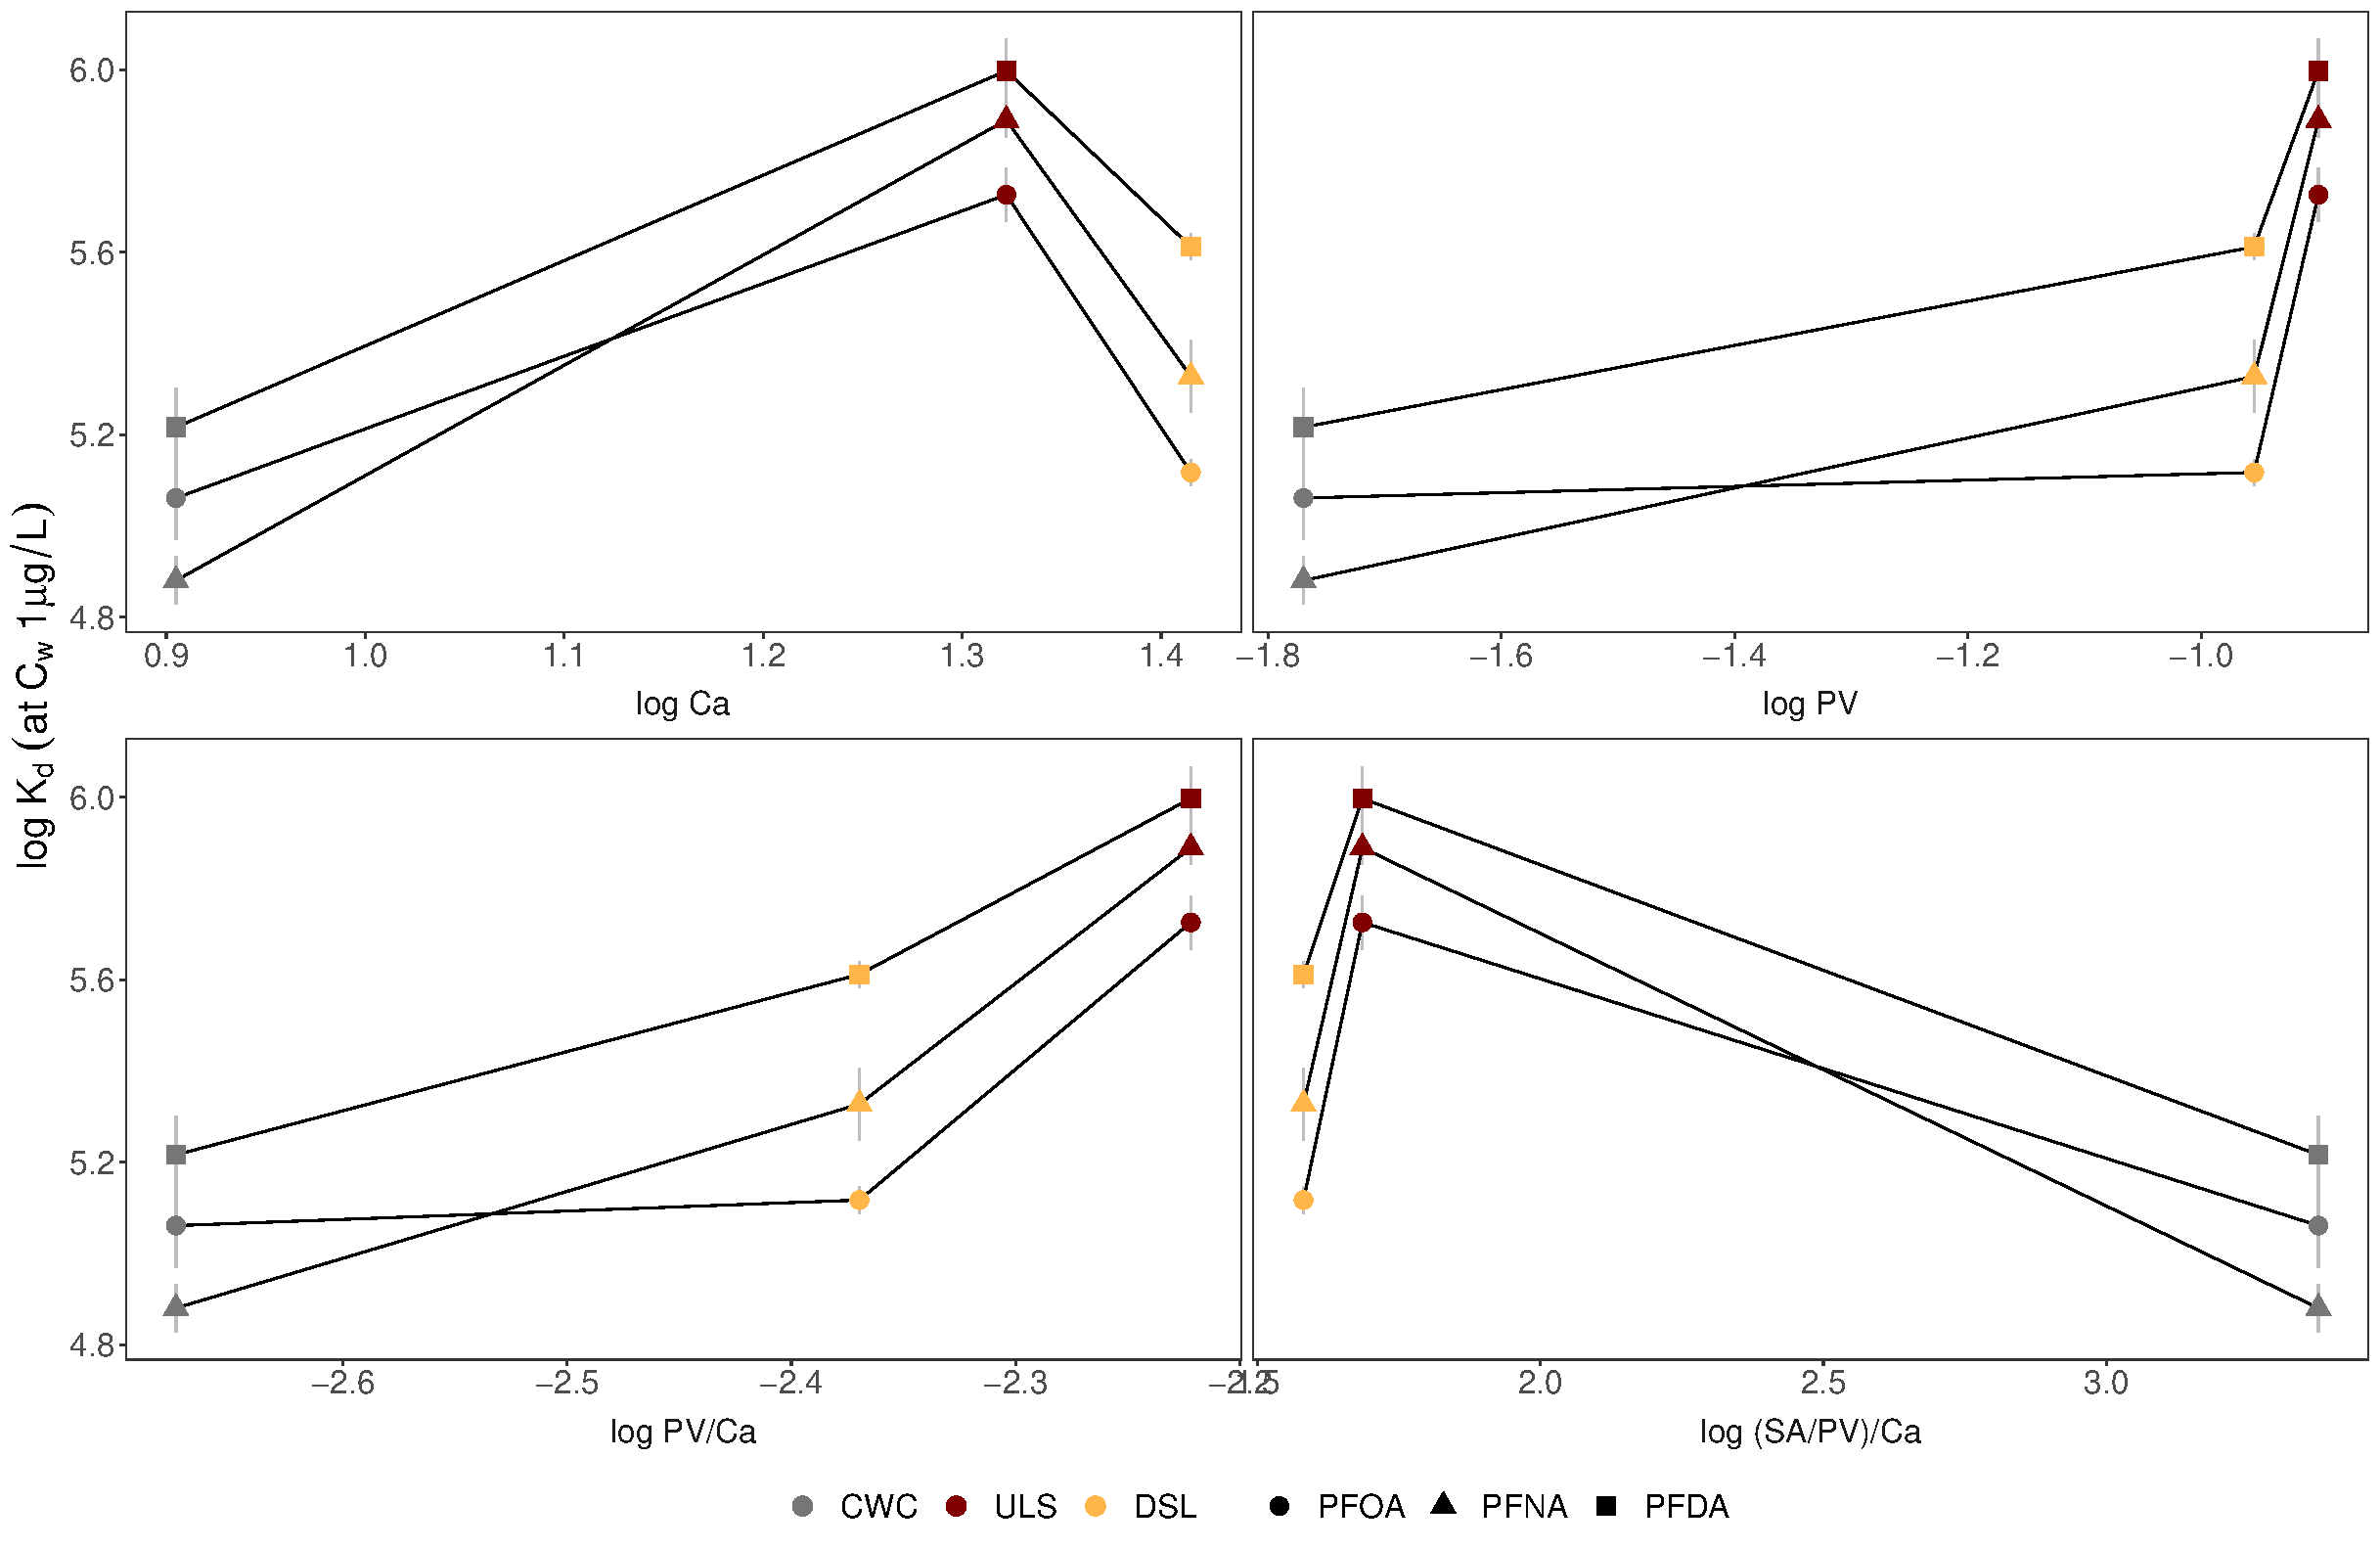
\includegraphics[width=0.8\textwidth]{R/figs/Correlation_SAPV_Ca_plot.pdf}
    \caption{The correlation of $\log~K_d$ vs. (a) log Ca (b) log PV (c) log PV/Ca (d) log (SA/PV)/Ca using BET for SA and BJH for PV by biomass feedstock. The points are discrete measurements, and the lines have been added to indicate trends. Error bars are the propagated standard error.}
    \label{fig:Kd_SAPV_Ca}
\end{figure}

%%%%%%%%%%%%%%%%%%%%%%%%%%%%%%%%%%%%%%%%%%%%%%%%%%%%%%%%%%%%%%%%%%%%%%%%%%%%%%%%%%%%%%%%%%%%%%%%%%%%%%%%%%%%%%%%%%%%%
%%%%%%%%%%%%%%%%%%%%%%%%%%%%%%%%%%%%%%%%%%%%%%%%%%%%%%%%%%%%%%%%%%%%%%%%%%%%%%%%%%%%%%%%%%%%%%%%%%%%%%%%%%%%%%%%%%%%%
%%%%%%%%%%%%%%%%%%%%%%%%%%%%%%%%%%%%%%%%%%%%%%%%%%%%%%%%%%%%%%%%%%%%%%%%%%%%%%%%%%%%%%%%%%%%%%%%%%%%%%%%%%%%%%%%%%%%%

\section{Sorption attenuation by soil and PFCA cocktail}
This section discusses sorption attenuation for the different batch test categories that were prepared (\cref{fig:batchtests_flowchart}). The categories were: 

\begin{itemize}
    \item \textbf{BC single}: biochar-water spiked with single PFCAs
    \item \textbf{BC mixed}: biochar-water spiked with a PFCA cocktail
    \item \textbf{BC soil single}: soil-biochar-water spiked with single PFCAs
    \item \textbf{BC soil mixed}: soil-biochar-water spiked with a PFCA cocktail
    \item \textbf{Soil single}: soil-water spiked with single PFCAs
    \item \textbf{Soil mixed}: soil-water spiked with a PFCA cocktail
\end{itemize}

\cref{subfig:C10} shows the $K_d$-values for the different batch test categories (BC single, BC soil single, BC soil mixed, BC mixed, soil single, and soil mixed) spiked with the same concentration of each compound at the highest spike point, SC10 (\cref{tab:spikeConcentrations}). $K_d$ for the biochar-soil batch tests has not been corrected for the amount sorbed by soil itself due to inconsistent results for the $K_d$ in soil (see \cref{appSec:Sorption}, \cref{apptab:attenuation} for soil $K_d$'s). Therefore, $K_d$ for BC soil single, BC soil mixed and BC mixed represent the collective partitioning coefficients for biochar and soil. The sandy soil used has poor sorption affinity, with a mean $\log~K_d$ value of 2.47, versus a $\log~K_d$ of, for example, 6.06 for singly-spiked PFDA to ULS-water. The total concentration of C5-C10 spiked at SC10 was 7.8 mg/L for the BC cocktail, and 10.8 mg/L for the BC soil cocktail. There is a 3 mg/L difference between these two because the cocktail batch tests were spiked in two different ways (described in \cref{sec:S-BC}). The cocktail consisted of 2.5\% PFPeA, 7.7\% PFHxA, 1.4\% PFHpA, 18.2\% PFOA, 21.3\% PFNA, and 48.8\% PFDA. Since the relative ratios of the compounds vary, a trend for attenuation with chain length cannot be derived. However, the relative $K_d$-values of each batch test category, as well as comparisons between biochar samples, yield interesting results. This way of comparing $K_d$-values for the same compound across biochar samples was decided to be the simplest way of comparing partitioning of the same compound across biochar samples because the initial concentrations ($C_i$) were constant.

In \cref{subfig:C10}, the drop in $\log~K_d$ from $\log~K_d$ for BC single represents how much the resulting partition coefficient for each batch test category is affected by the presence of soil and a PFCA cocktail. Fouling, together with attenuation, are terms used to discuss the weakening of sorbent sorption by natural organic matter or competing contaminants \citep{Werner2006}. For all compounds, the presence of a mixture is responsible for the highest drop in $\log~K_d$. Overall, $\log~K_d$ decreases in the following order: BC single $>$ BC soil single $>$ BC soil mixed $>$ BC mixed $>$ soil single and mixed. Attenuation appears to be similar for all biochars as the points for each batch type align parallel, at least for the higher-quality results for PFOA, PFNA, and PFDA. This trend shows that the mixed systems have greatest attenuation, where sorption is up to two orders of magnitude weaker than the reference. This means that sorption is non-linear at high concentrations, something which will be discussed further in \cref{sec:non-linearity}. These results are in line  with previous literature \citep{deng2010removal, zhou2010sorption}.

\subsection{Attenuation factors}
\cref{subfig:AF} shows the attenuation factors (AF) for each batch test category, defined as:

\begin{equation} \label{eq:AF}
    AF = \frac{K_{d,BC single}}{K_{d,x}}
\end{equation}

where the numerator, $K_{d,x}$, is the mixed, soil mixed, or soil single batch test sample partition coefficient. AFs for PFPeA, PFHxA and PFHpA were removed due to lack of consistent results. Lowest attenuation (lowest AFs) was measured for PFOA-BC-soil, where AFs were 0.65, 0.71, and 0.90 for CWC, DSL, and ULS respectively. A table with all AFs are in \cref{apptab:attenuation}. It appears that ULS, which has the highest sorption, also has the highest attenuation. There are two possible explanations for this trend: 1) The most attractive sorption sites on ULS are limited and easily blocked, and 2) In addition to the strong competition for the most attractive sorption sites described in 1), the reported $K_d$-values for the batch tests with soil are average values for sorption of biochar and soil together. The closer the sorption of the char is to the soil, the less the apparent attenuation effect. Since ULS has the highest difference in $K_d$ compared to the soil, attenuation is enhanced.

Highest attenuation were measured for the cocktail samples, with minor variance between the BC soil mixed and BC mixed samples. AFs are in the range 0.993-0.84 which means that sorption has been reduced by 84-99\%. This suggests that the total concentration of the cocktail is responsible for saturating sorption sites almost completely, and that the presence of soil in this case does not contribute to additional fouling. Overall, \cref{fig:C10_AF} shows that attenuation by the cocktail is more significant than attenuation by soil. This can mean two things: 1) The soil does not block biochar sorption sites, or 2) The soil, which has a $\log~K_d$ of 2.6 $\pm$ 2.0, sorbs some of the PFCAs that have been blocked from sorption onto the biochar. 

Colored filtrate and humus aggregation seen during analysis of the soil batch tests indicate that co-sorption to organic matter (OM) in the BC-soil-water batch test is likely (see \cref{sec:S-BC}. The soil used was a sandy soil with 1.3 \% TOC (details on soil properties is in \cref{sec:Soil}). By the co-existence of OM and dissolved organic carbon (DOC), sorption attenuation occurs by a combination of competitive and weaker sorption of PFAS to OM and DOC, and the competitive sorption of OM to biochar. Large humic acids (300-600 nm) clog the pores, preventing diffusion of PFAS \citep{Cornelissen2006,kluvcakova2018size}. Furthermore, the size of the organic molecules is a critical factor as humic molecules whose size is similar to that of PFAS are responsible for the highest competition \citep{du2014adsorption}. Given that size fractionation was not investigated in this study, the effect of differences of size for humic acids can only be discussed in theory.

\begin{figure}
    \centering
        \begin{subfigure}[]{\linewidth}
            \centering
            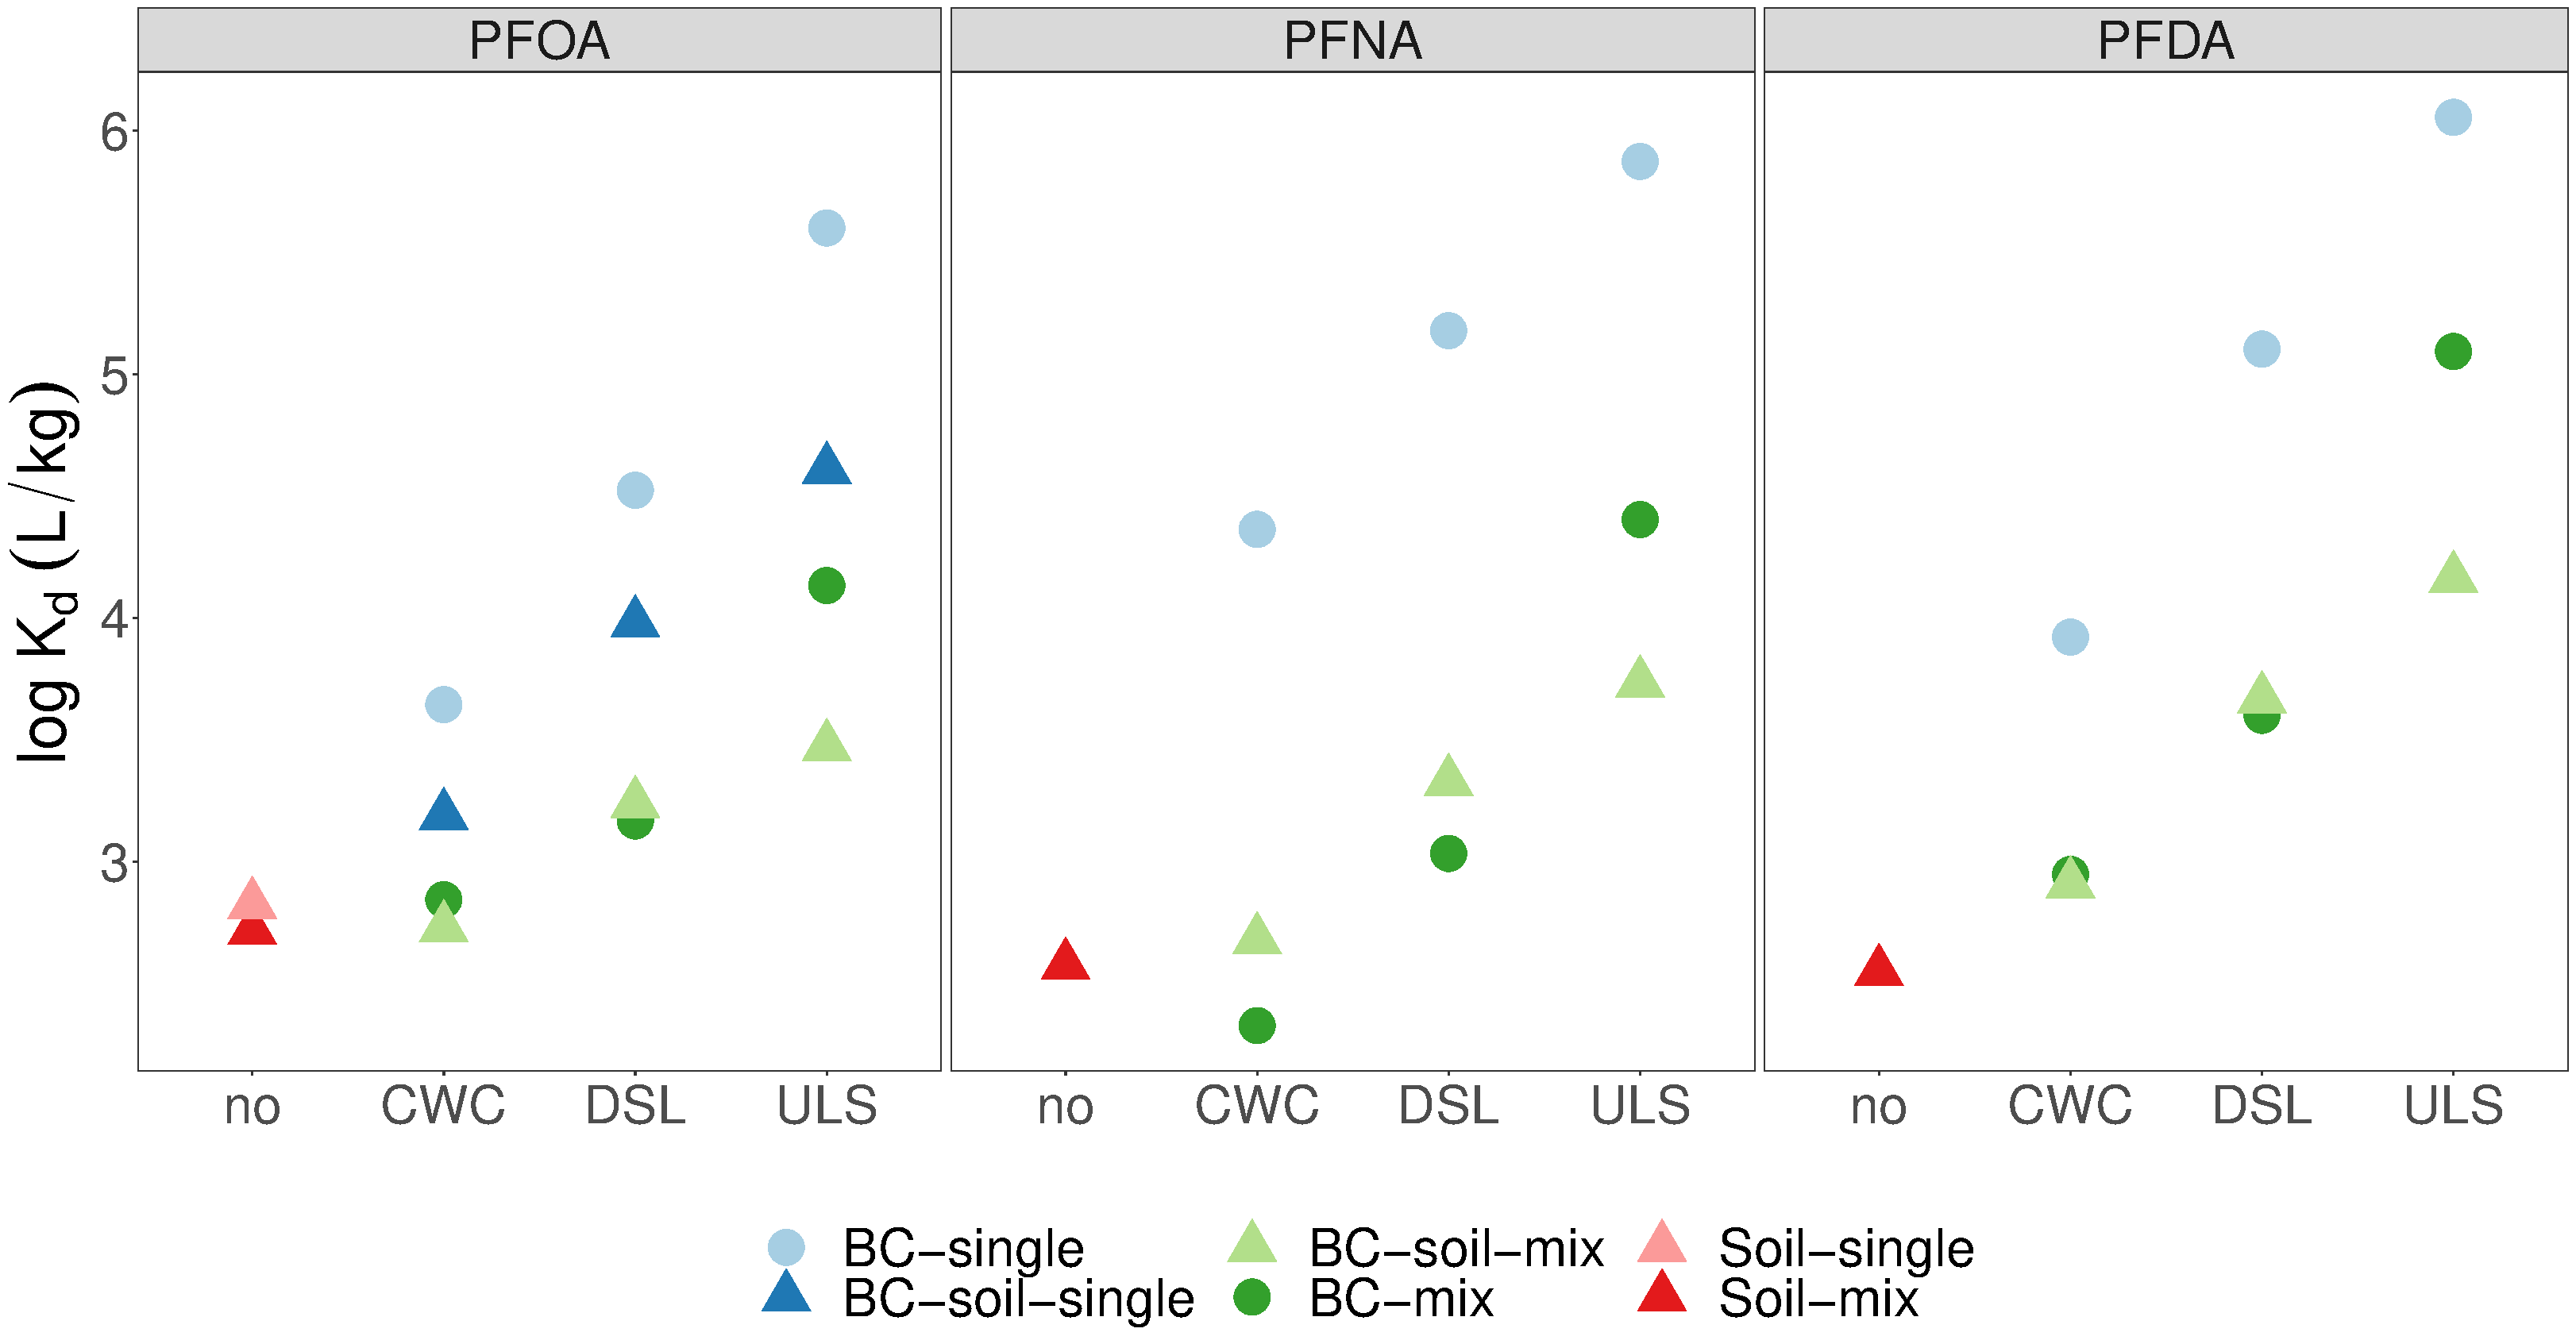
\includegraphics[width=0.75\textwidth]{R/figs/C10.pdf}
            \subcaption{$\log~K_d$ for each target compound spiked at SC10 (191, 330, 117, 1 953, 1 409, and 3 830 \textmu g L\textsuperscript{-1} for C5-C10, respectively) for the different biochar feedstocks (CWC, DSL, ULS) and soil only (no).}
            \label{subfig:C10}
        \end{subfigure}
        \begin{subfigure}[]{\linewidth}
            \centering
            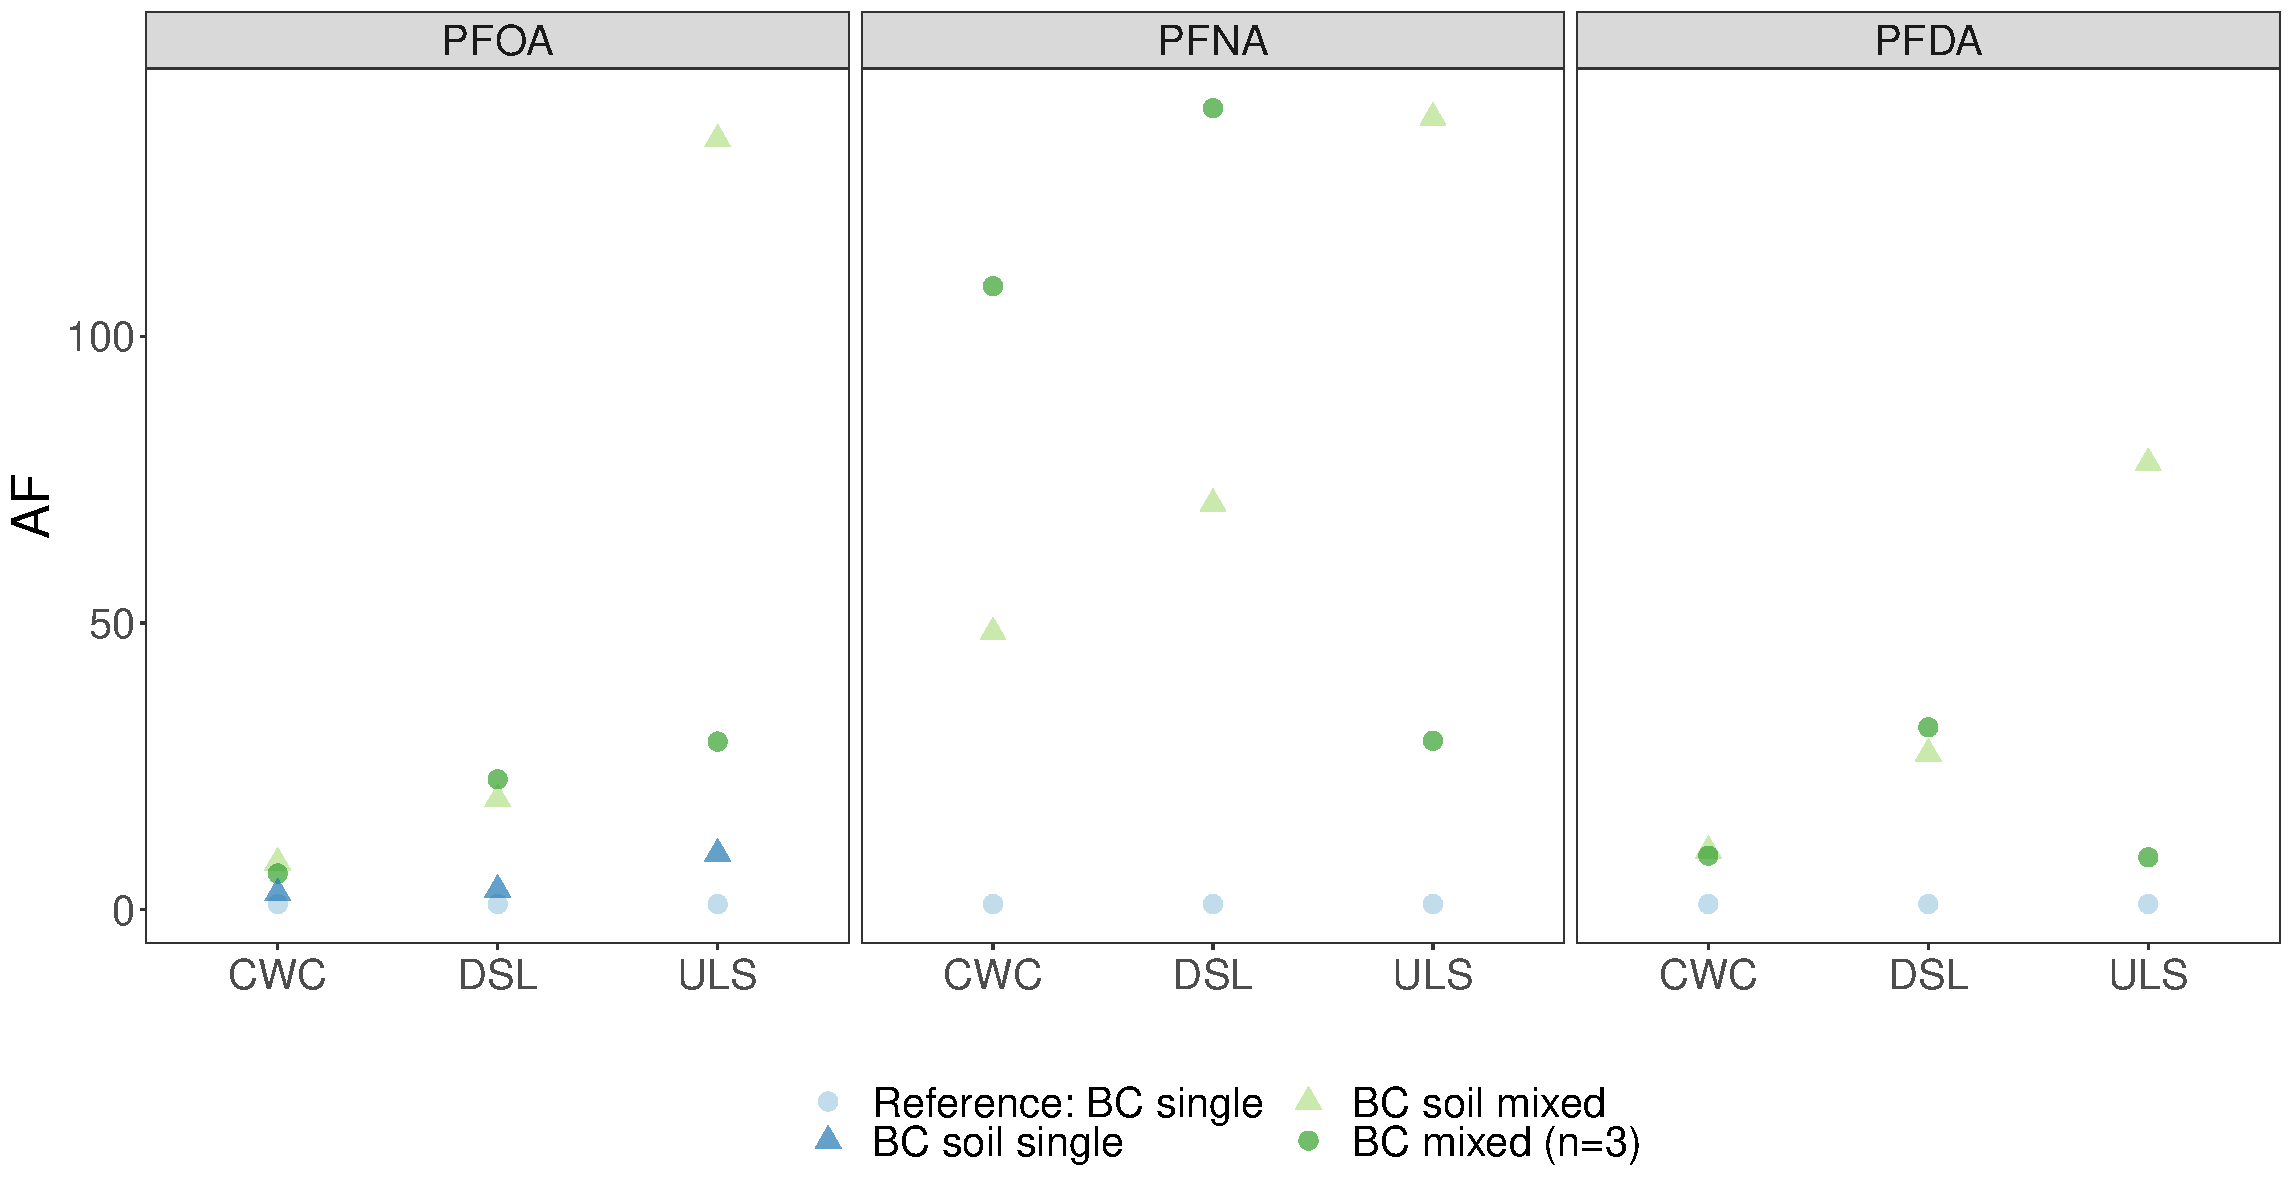
\includegraphics[width=0.75\textwidth]{R/figs/Attenuation_factors_C10_OND.pdf}
            \subcaption{Attenuation factors at SC10 for C8-C10 calculated as 1 - the fraction of $K_d$ for mixed/soil/mixed and soil samples over $K_d$ of BC single (\cref{eq:AF}). BC cocktails are spiked with 7.8 mg/L total PFCA and BC soil cocktails with 10.8 mg/L (the difference is explained in the corresponding section). See \cref{tab:spikeConcentrations} for spike concentrations used for each PFCA in the single-spike and cocktail-spike batch tests.}
            \label{subfig:AF}
        \end{subfigure}  
    \caption{Reduction in \textbf{(a)} $\log~K_d$ at SC10 and \textbf{(b)} attenuation factors at SC10.}
    \label{fig:C10_AF}
\end{figure}

\subsection{Sorption attenuation of PFOA isotherms}
\cref{fig:PFOA_attenuation} shows the effect of attenuation on the PFOA isotherms for BC soil single and BC soil mixed. The isotherms were spiked with the same $C_i$ as BC single, but only six of the ten points were selected for the attenuation isotherms (\cref{sec:S-BC}. For all biochars, BC single has the highest sorption, followed by BC soil single, and BC soil mixed. This trend gives a good indication of the order of factors that influence attenuation, and is consistent with the results discussed earlier in this section. The isotherms have similar $C_s$ concentrations, but varying $C_w$, depending on sample type. Due to pore blocking and competitive sorption, more sorbate in solution is needed to push the same amount of molecules onto the solid phase in the presence of soil. This effect can be further enhanced by the presence of both soil and a cocktail since this isotherm has the highest $Cw$ and lowest $C_s$. This is due to the fact that PFCAs with longer chain lengths (PFNA and PFDA) have an advantage over PFOA when competing for sorption sites \citep{Sormo2021}. Consistent with \cref{fig:C10_AF}, the cocktail attenuation effect is more significant than attenuation by soil. Parallel isotherms mean that attenuation is the same across the whole concentration range, as, for instance, between BC single and BC soil single for ULS. For some isotherms, attenuation is minimal at low concentrations and increases with increasing spike concentration. This is the case for the DSL isotherms, something that can be explained by the non-linear sorption at higher concentrations. So, when spike concentration increases, sorption attenuation also increases. 

\begin{figure}[htb]
    \centering
    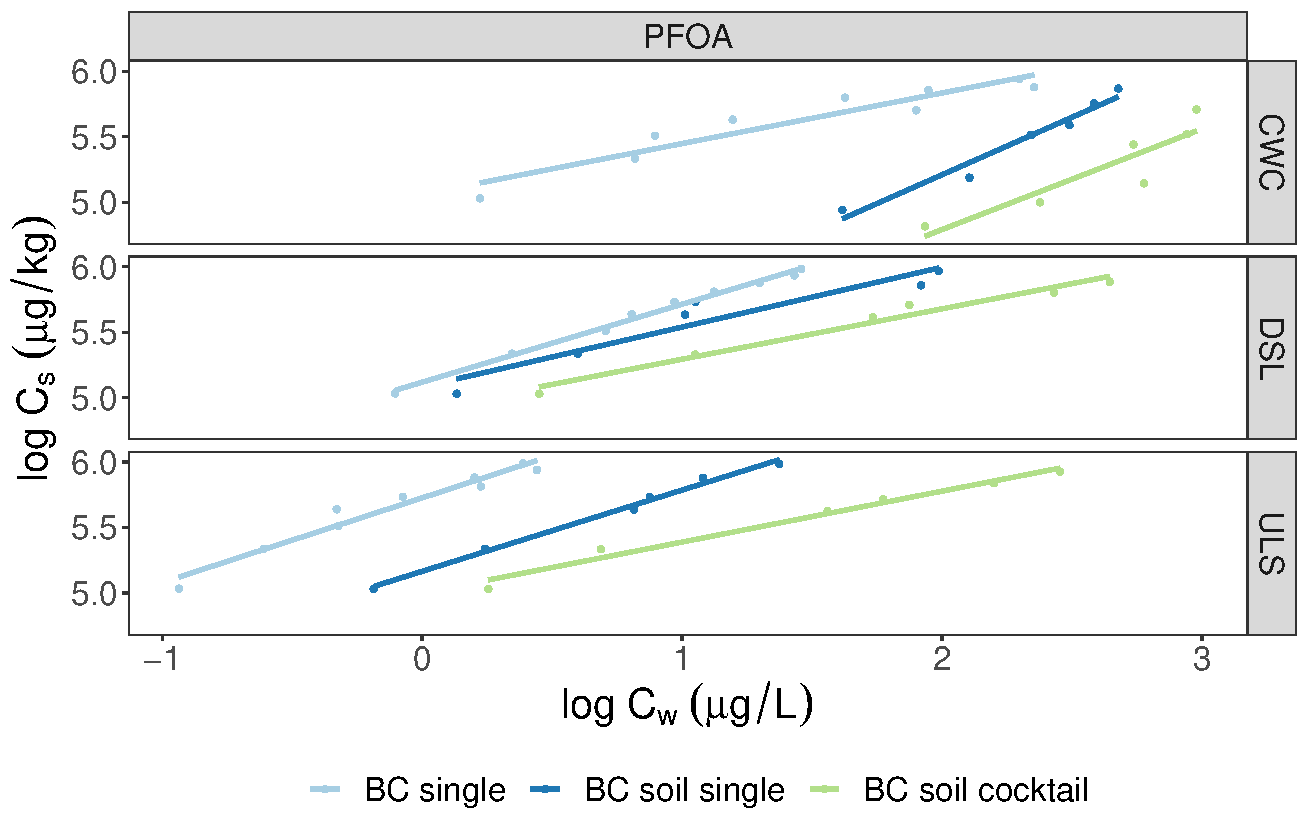
\includegraphics[width=0.8\textwidth]{R/figs/Attenuation_isotherms_PFOA.pdf}
    \caption{Sorption isotherm comparison for PFOA single-compound spike in biochar (BC single), single-compound spike in soil-biochar (BC soil single), and PFOA spiked in a cocktail in soil-biochar showing attenuation by soil and competing congeners.}
    \label{fig:PFOA_attenuation}
\end{figure}

\subsection{Freundlich sorption non-linearity}\label{sec:non-linearity}
The non-linear sorption isotherms for PFOA in \cref{fig:PFOA_nonlinear} shows how sorption is attenuated at higher concentrations, and how attenuation changes in the presence of soil and soil with cocktail. When a linear model is derived from applying the $\log$ of each axis, the slope ($n_F$) represents how linear the isotherm is within the concentration interval achieved (\cref{sec:models}). The resulting Freundlich coefficients ($\log~K_F$ and $n_F$) for PFOA are given in \cref{tab:PFOA_Freundlich}, and the remaining compounds are in \cref{appSec:Sorption}\cref{apptab:summary_stats_all}. Two general conclusions can be drawn from these figures: 1) Attenuation is higher in the presence of soil, and even higher when soil and cocktail are added together. And 2) The concentration ranges for some of the isotherms are too narrow to properly determine representative Freundlich coefficients for a wider concentration range. Therefore, conversion of $\log~K_F$ to either higher or lower units will be associated with greater uncertainty. 

All BC single isotherms have $n_F<1$. This indicates that the concentration interval achieved shows some degree of attenuation (\cref{tab:summary_stats_single}. This is consistent with other studies where sorption to biochar have $n_F$-values, typically, around 0.3-0.7 \citep{Cornelissen2005}. Both concentration interval and $n_F$ should be considered together in order to make suggestions about the sorption capacity of biochars. \cref{fig:nonlinear_OND} shows the non-linear BC-single isotherms for PFOA, PFNA and PFDA, where the degree of non-linearity is more easily visualized than the $n_F$-values alone. For example, \cref{fig:nonlinear_OND} shows that the CWC isotherms have more attenuation than DSL and ULS, and that $C_w$s have measurements across a wider concentration range. This is consistent with the lower $\log~K_F$s found for CWC. \cref{fig:nonlinear_OND} also shows that the isotherms for PFNA-DSL and PFNA-ULS are nearly linear, and span aqueous concentrations only within the same order of magnitude. Higher spike concentrations, or lower BC dosages, should have been used in order to get isotherms that cover the regions of attenuated sorption for these biochars and compounds. However, this information itself indicates that sludge biochars have higher sorption capacities than CWC.  

The concentration range achieved for $C_w$ for the sorption isotherms was an average of 1.3 $\log$ units, in contrast to the desired concentration range over 4 $\log$ units. Poor signals were achieved for the SC1 points and were removed from the data analysis. This resulted in the spike concentration interval being reduced to two orders of magnitude \cref{tab:spikeConcentrations}. In retrospect, spike concentrations at each $\log$ unit should have been selected instead of spreading the ten concentrations evenly across the concentration range. For the short-chain compounds (PFPeA and PFHxA), correlations were poor. This resulted in higher standard errors, and some slopes that have $n_F>1$, which is unrealistic (PFHxA-DSL: n=1.11 and PFHpA-ULS: 1.08). However, the standard error is also high ($\pm$ 0.11 for both) and can account for this abnormality. Poor sorption affinity of PFPeA and PFHxA to biochar may explain the poor correlations. The CWC isotherms had the widest concentration intervals for $C_w$. This can be understood by the fact that CWC is the weakest sorbent of the three biochars studied.  

Electrostatic interactions between PFCAs and sediment can contribute to enhancing saturation of the adsorption sites as well as intermolecular electrostatic repulsion between individual molecules \citep{higgins2006sorption,yin2022insights}. \cite{yin2022insights} suggests four explanations for why sorption of PFCAs to biochar is non-linear: 1) the complex composition of biochar with negative, positive and neutral charges within same matrix, 2) successive saturation of adsorption sites, 3) electrostatic interactions between the PFASs and sediment, and 4) electrostatic repulsion from negatively charged carboxylate groups.

\begin{table}
\caption{Freundlich sorption parameters and standard errors for the PFOA isotherms. Freundlich coefficients for the soil samples are the collective partition coefficients for soil and biochar because $K_d$ for soil alone was not accurate enough. All $K_F$ data are in units of $\mathrm{(\mu g/kg)/(\mu g/L)^{n_F}}$.}
\centering
\adjustbox{max width=\textwidth}{%
\begin{threeparttable}
\label{tab:PFOA_Freundlich}
\begin{tabular}{lllllll} \toprule
\multicolumn{1}{c}{Compound} & \multicolumn{1}{c}{Biochar} & \multicolumn{1}{c}{type} & \multicolumn{1}{c}{$\log~K_F$} & \multicolumn{1}{c}{$n_F$} & \multicolumn{1}{c}{$r^2$} & \multicolumn{1}{c}{$p$} \\ \midrule
PFOA & CWC & BC\_S\_mix  & 3.25 ± 0.5 & 0.77 ± 0.2 & 0.82 & * \\
PFOA & CWC & BC\_S\_sing & 3.45 ± 0.2 & 0.88 ± 0.09 & 0.96 & ** \\
PFOA & CWC & BC\_sing    & 5.06 ± 0.08 & 0.39 ± 0.05 & 0.90 & *** \\
PFOA & DSL & BC\_S\_mix  & 4.91 ± 0.06 & 0.39 ± 0.03 & 0.97 & *** \\
PFOA & DSL & BC\_S\_sing & 5.08 ± 0.1 & 0.46 ± 0.08 & 0.90 & * \\
PFOA & DSL & BC\_sing    & 5.12 ± 0.02 & 0.60 ± 0.02 & 0.99 & *** \\
PFOA & ULS & BC\_S\_mix  & 5.00 ± 0.05 & 0.39 ± 0.03 & 0.98 & *** \\
PFOA & ULS & BC\_S\_sing & 5.16 ± 0.03 & 0.62 ± 0.03 & 0.99 & *** \\
PFOA & ULS & BC\_sing    & 5.73 ± 0.02 & 0.65 ± 0.05 & 0.95 & *** \\ \bottomrule
\end{tabular}
\begin{tablenotes}
\item Significant codes: *** $\sim$ 0.001, ** $\sim$ 0.01, * $\sim$ 0.05
\end{tablenotes}
\end{threeparttable}}
\end{table}

\begin{figure}
    \centering
    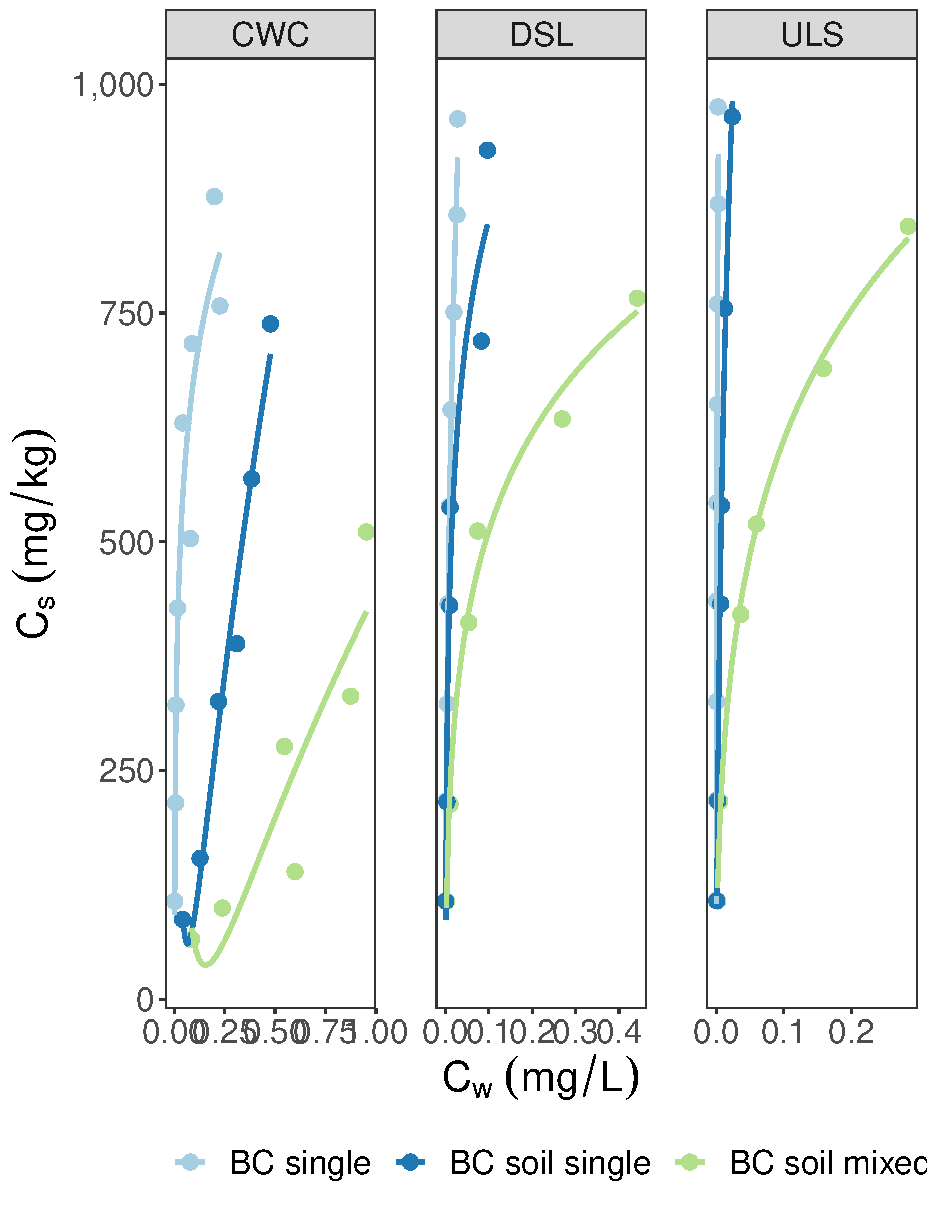
\includegraphics[width=0.8\textwidth]{R/figs/PFOA_linear.pdf}
    \caption{Attenuation isotherms for PFOA in BC-single, BC-mixed and BC-soil-mixed fitted by a polylogarithmic function.}
    \label{fig:PFOA_nonlinear}
\end{figure}

\begin{figure}
    \centering
    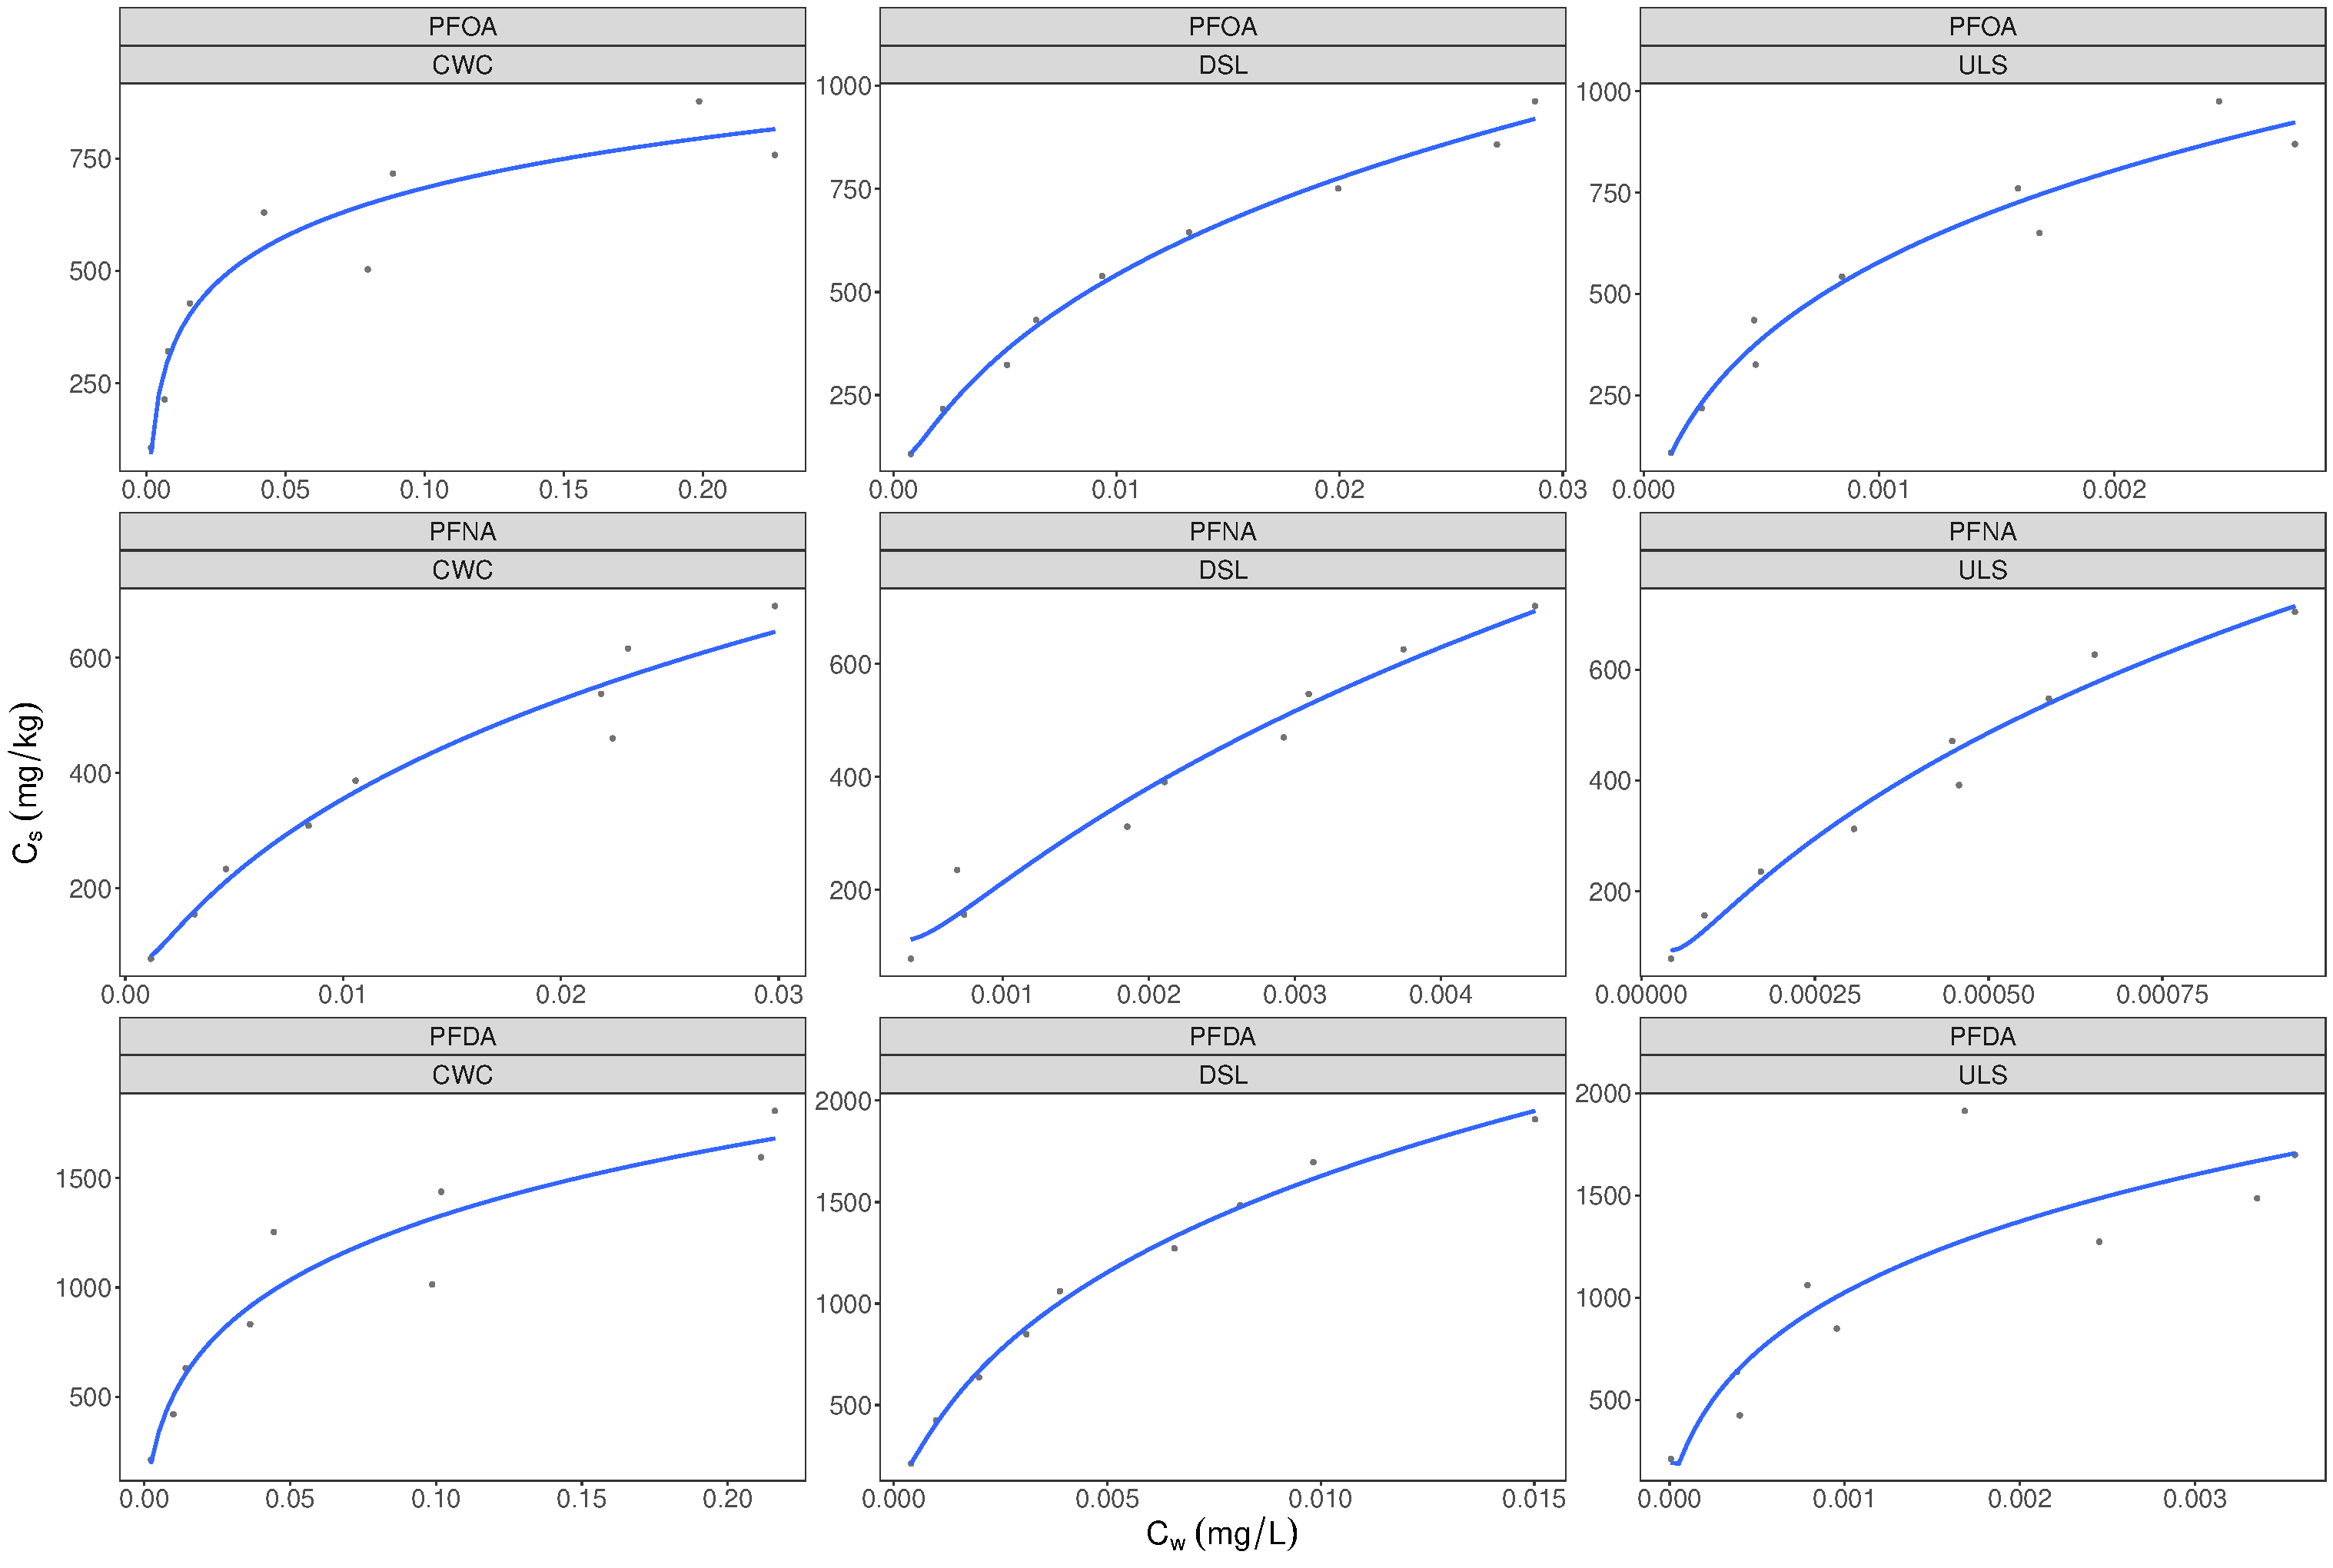
\includegraphics[width=\textwidth]{R/figs/BC_single_attenuation.pdf}
    \caption{Attenuation isotherms for single-spike PFOA, PFNA and PFDA with CWC, DSL, and ULS fitted by a polylogarithmic function.}
    \label{fig:nonlinear_OND} 
\end{figure}


%%%%%%%%%%%%%%%%%%%%%%%%%%%%%%%%%%%%%%%%%%%%%%%%%%%%%%%%%%%%%%%%%%%%%%%%%%%%%%%%%%%%%%%%%%%%%%%%%%%%%%%%%%%%%%%%%%%%%%%%%%%%%%%%%%%%%%%%%%%%%%%%%%%%%%%%%%%%%%%%%%%%%%%%%%%%%%%%%%%%%%%%%%%%%%%%%%%%%%%%%%%%%%%%%%%%%%%%%%%%%%%%%%%%%%%%%%%%%%%%%%%%%%%%%%%%%%%%%%%%%%%%%%%%%%%%%%%%%%%%%%%%%%%%%%%%%%%%%%%%%%%%%%%%%%%%%%%%%%%%%%%%%%%%%%%%%%%%%%%%%%%%%%%%%%%%%%%%%%%%%%%%%%%%%%%%%%%%%%%%%%%%%%%%%%%%%%%%%%%%%%%%%%%%%%%%%%%%%%%%%%%%%%%%%%%%%%%%%%%%%%%%%%%%%%%%%%%%%%%%%%%%%%%%%%%%%%%%%%%%%%%%%%%%%%%%%%%%%%%%%%%%%%%%%%%%%%%%%%%%%%%%%%%%%%%%%%%%%%%%%%%%

\section{Soil properties}\label{sec:Soil}
The soil used in the batch tests was classified as a fine sand (0.1 to 0.3 mm) with 1.3 \% TOC (pH 5.38 $\pm$ 0.02, CEC 2.63 $\pm$ 0.06 meqv 100 g\textsuperscript{-1}). Total element concentrations and exchangeable ion concentrations are in \cref{appSec:elements}, \cref{apptab:soil}. Soil extraction showed no native PFCAs present. 

Before filtration of the batch tests with soil, each sample category (CWC-soil, DSL-soil, ULS-soil and soil only), despite being centrifuged, contained different degrees on suspended particles. This made it difficult to filter the samples that contained the most suspended particles. Filtration led to clogged filters that had to be changed up to three times per sample. The resulting filtrates varied in color \cref{fig:DOC}. These differences can be attributed to different amounts of dissolved organic carbon (DOC). The sludge biochar-soil samples were more transparent than soil only and soil-CWC. The remarkable difference in DOC is attributed to DOC complexation with inorganic species present in the sludge chars, but not in CWC. Frequently clogged filters likely resulted in reduced filter pore size associated with the fact that some DOC was retained. This may have led to underestimating $C_w$, and thereby overestimating $K_d$ for soil which, in turn, became an issue when deriving $K_F$ for the biochar in these samples using \cref{eq:FreundLinSoil4}. Filter blanks were only prepared for BC-water samples that showed no significant effect (see \cref{apptab:FB}). Hence, the effect of reduced filter size by clogging cannot be quantified. In summary, the results and observations from the BC soil batch tests indicate that sewage sludge biochar binds DOC, and DOC in the filtrate is potentially responsible for an overestimation of $C_w$, and hence, underestimation of $K_{d,s}$. 

\begin{figure}
    \centering
    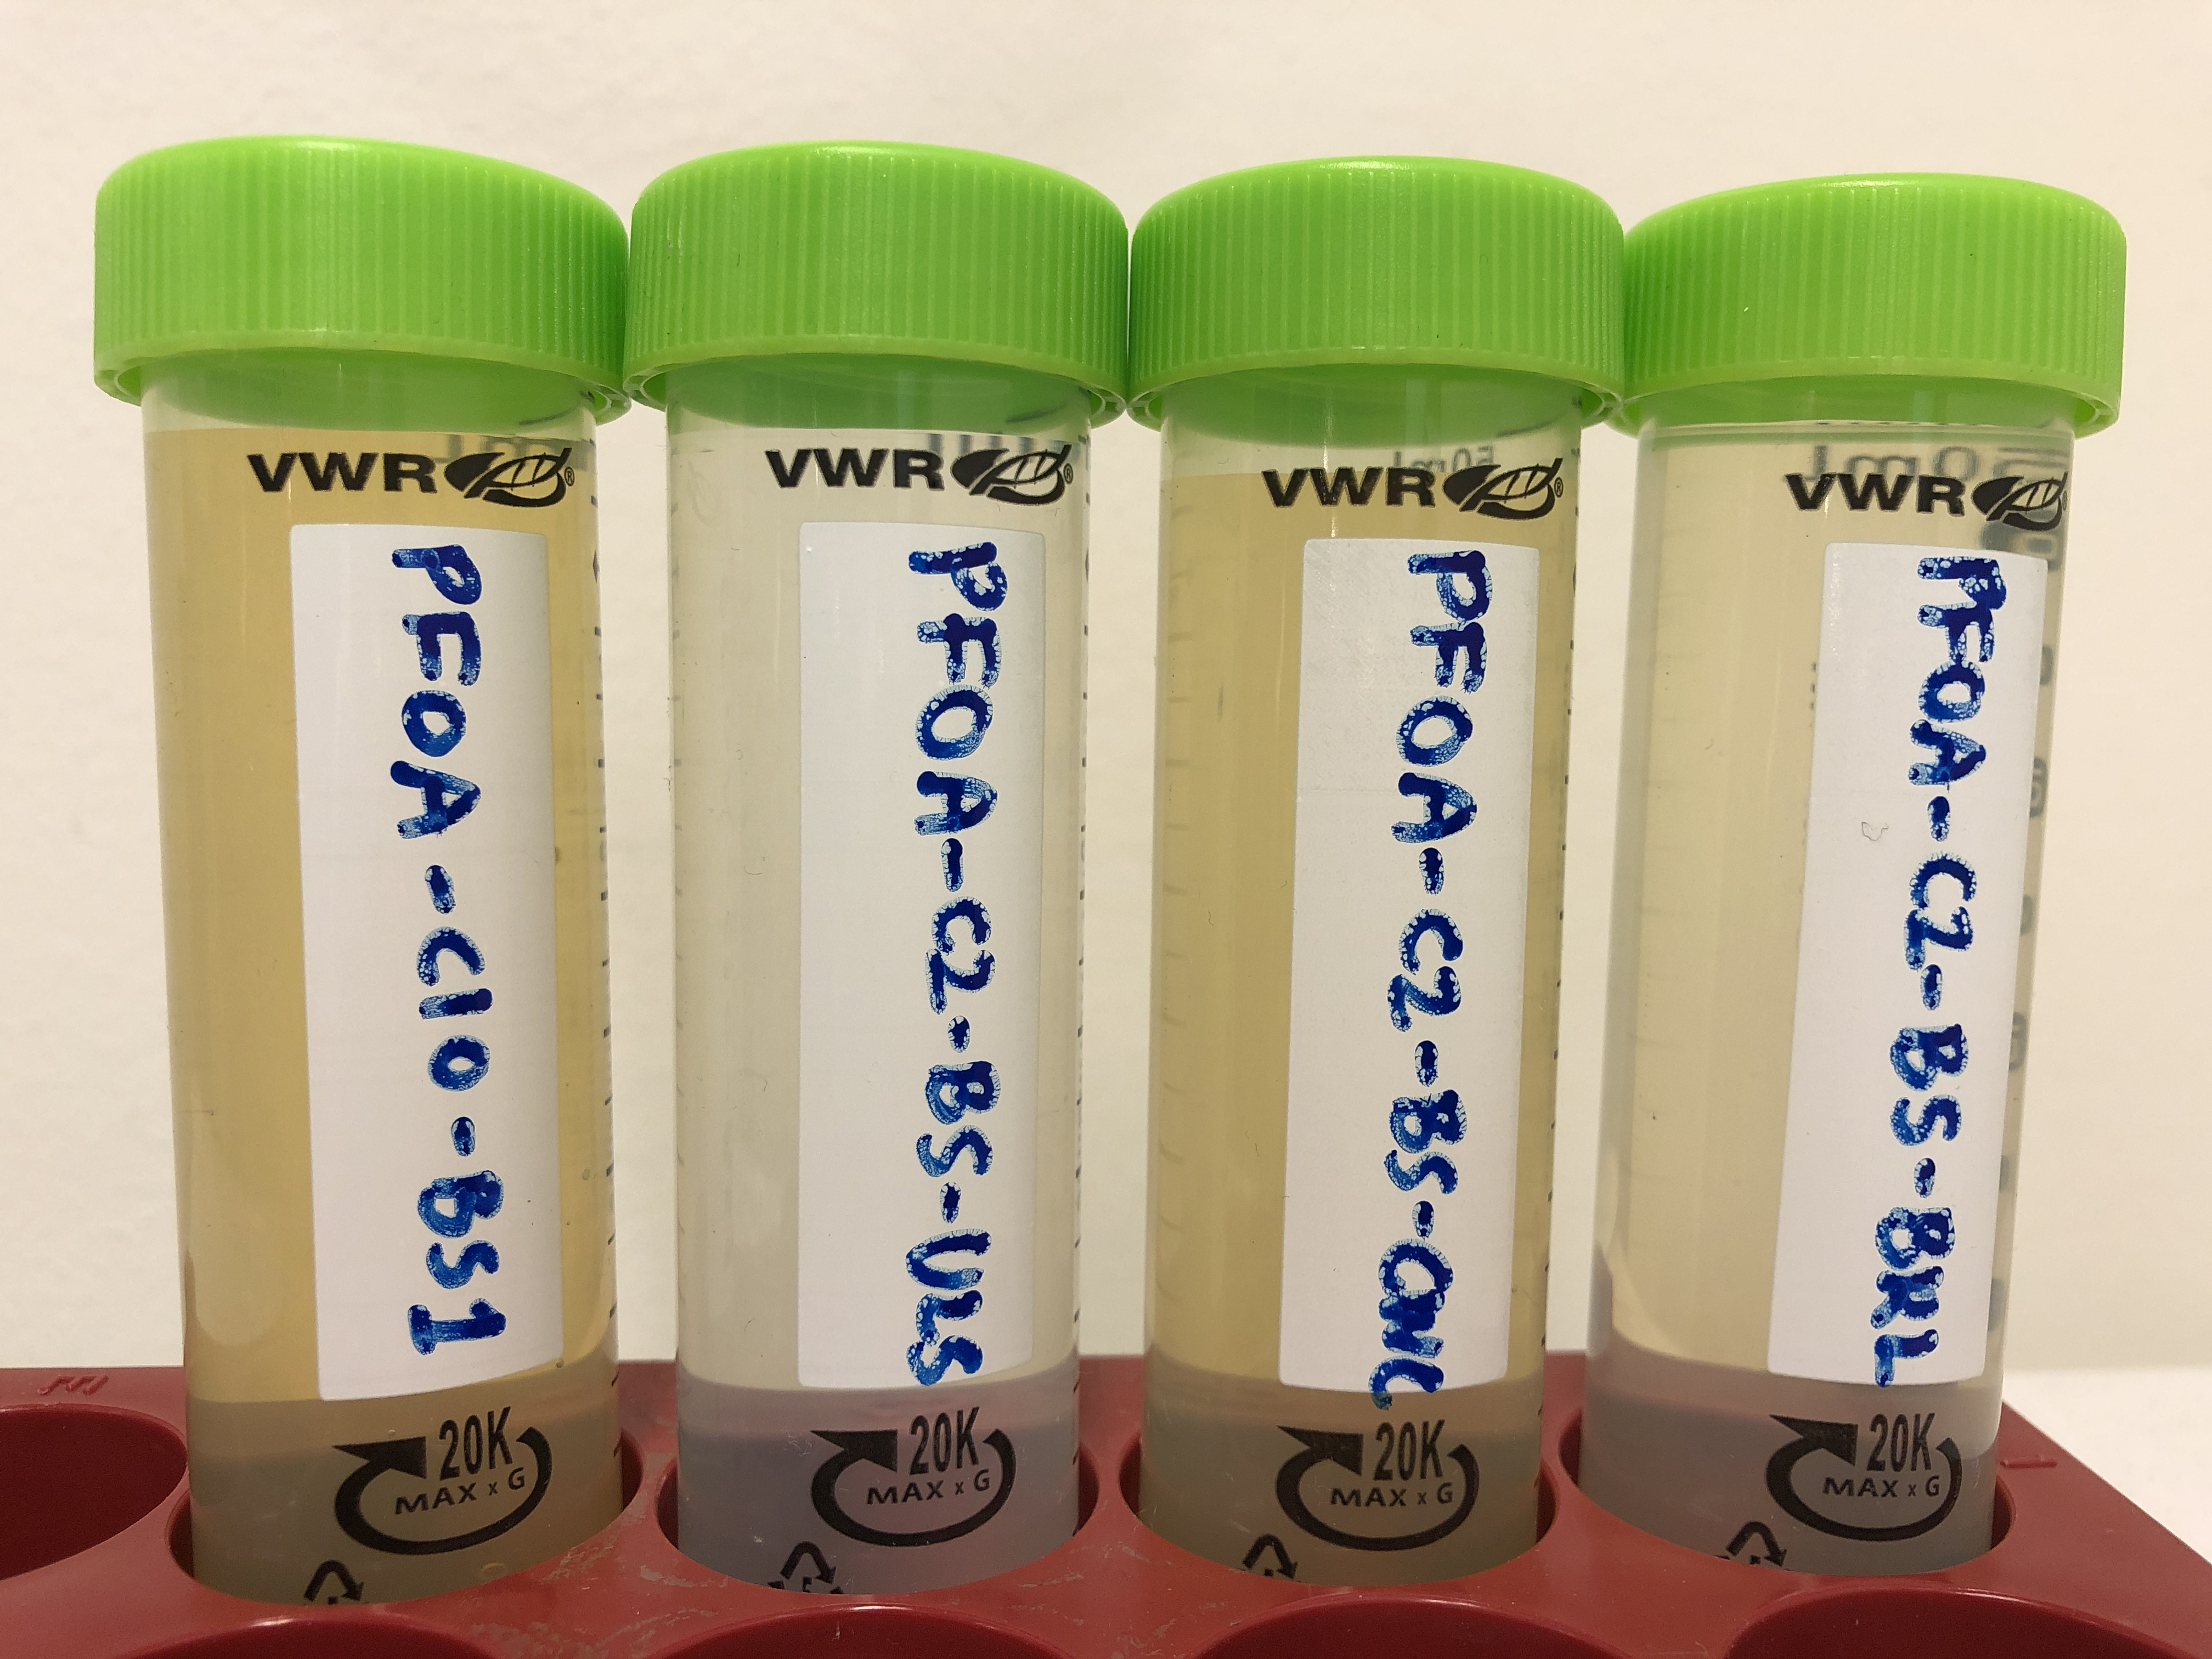
\includegraphics[width=0.7\textwidth]{Bilder/Samples/Filtrate_DOC.JPG}
    \caption{Color of filtrate for each biochar batch test. From left to right: soil only, soil+ULS, soil+CWC, and soil+DSL (BRL = DSL).}
    \label{fig:DOC}
\end{figure}

%%%%%%%%%%%%%%%%%%%%%%%%%%%%%%%%%%%%%%%%%%%%%%%%%%%%%%%%%%%%%%%%%%%%%%%%%%%%%%%%%%%%%%%%%%%%%%%%%%%%%%%%%%%%%%%%%%%%%
%%%%%%%%%%%%%%%%%%%%%%%%%%%%%%%%%%%%%%%%%%%%%%%%%%%%%%%%%%%%%%%%%%%%%%%%%%%%%%%%%%%%%%%%%%%%%%%%%%%%%%%%%%%%%%%%%%%%%
%%%%%%%%%%%%%%%%%%%%%%%%%%%%%%%%%%%%%%%%%%%%%%%%%%%%%%%%%%%%%%%%%%%%%%%%%%%%%%%%%%%%%%%%%%%%%%%%%%%%%%%%%%%%%%%%%%%%%

\section{Potential for commercializing sludge chars as sorbents}
The sorption capacity of the sewage sludge biochars was tested in a controlled laboratory environment, with a low-TOC soil, and artificially spiked PFCAs. Therefore, the results from this research does not account for the heterogeneity in factors like different soil types and organic matter contents, diversity of organic contaminants, and variations in PFAS concentration levels that may influence sorption strength. However, the results show that sewage sludge biochars bind PFCA strongly, especially for the long-chain compounds at concentrations that are many times higher than actual environmentally relevant concentrations. Separate investigations should also be conducted to determine the sorption capacity of biochars, work that is especially important to establish how long a carbon filter for wastewater treatment can be used. Care must be taken when applying a highly contaminated feedstock to make sure no heavy metals are leached the environment and no additional PFAS is released from the sewage sludge. Results from a parallel project with this thesis will hopefully be able to provide a fuller understanding of a range of issues, including gaseous pollution measurements, biochar PFAS content, and particulate matter measurements. The hope is that PFAS is eliminated at pyrolysis temperatures.

\subsection{Life cycle assessment (LCA) \label{sec:LCA}}
To assess the overall environmental impacts associated with pyrolysis of sewage sludge, research partners are currently working on a life cycle assessment (LCA). Factors such as GHG burden, energy inputs versus energy recovery, environmental impacts, and economic profitability are weighted in such an assessment \citep{huang2022comparative}. Generally, the highest energy demands are associated with moisture removal and heating of the pyrolysis chamber since burning of biomass without oxygen is endothermic \citep{mcnamara2016pyrolysis}. A recent LCA on pyrolysis of sewage sludge by \citep{huang2022comparative} reported that net energy recovery by biochar and bio-oil pyrolysis is more sustainable than conventional sludge treatment methods, and has the potential to generate acceptable levels of profit \cite{huang2022comparative}. The feedstocks used in the present research have highly different caloric contents, where DSL has the lowest caloric content because it already has been through anaerobic digestion for bio-gas production. If DSL can be introduced as a commercial sorbent, this will increase the LCA even further. More research is needed to look at the potential for using low-grade bio-oil and syn-gas byproducts from pyrolysis for something for/to ????. These byproducts share a range of drawbacks related to successfully integrating them into a circular economy: they often contain a good deal of water, emerging contaminants and varying concentrations of heavy metals.  

\subsection{Sustainable development goals (SDGs) \label{sec:SDGs}}
Several initiatives have been started related to the roles biochar can have in means to work towards reaching the United Nations (UN) Sustainable Development Goals (SDGs) \citep{SDGs2015} and the European Green Deal of 2020. The European Green Deal of July 14, 2021 set that biochar is a means to achieve the goal to make Europe the first climate neutral continent through economic means: biochar is a potential commercial product in a circular economy\footnote{\url{https://ec.europa.eu/info/strategy/priorities-2019-2024/european-green-deal/delivering-european-green-deal_en}}. The 4 per mille initiative - Soils for food security and climate, was launched by France during the UN climate change conference of December 2015 (COP21)\footnote{\url{https://www.4p1000.org/}}. The 4 per 1000 mission is to increase soil carbon stocks in the first 30-40 cm of soil by 4 \textperthousand  annually to complement what is necessary efforts to reduce GHG emissions globally. The goal is to scale biochar for global agricultural and remediation markets. If applied correctly, biochar can play an important role for carbon sequestration at the same time as serving as a soil amendment and fertilizer in agriculture. However, care must be taken because application of biochar in soil has shown to have a priming effect on soil native C by improving microbial populations, thereby increasing the decomposition rate of organic matter \citep{Ahmad2014}. The International Biochar Initiative (IBI) is a collaborative platform for science, industry, agriculture, government, and non-governmental organizations to spread awareness about the beenefits with biochar and develop biochar standards for safe and sustainable use\footnote{\url{https://biochar-international.org/about-ibi/}}. Initiatives related to the overarching project of this thesis (VOW\footnote{\url{https://www.ngi.no/eng/Projects/VOW-Valorization-of-Organic-Waste}}) include ZeroPM\footnote{\url{https://zeropm.eu}}, EarthResQe\footnote{\url{https://www.nmbu.no/en/services/centers/earthresque}}, SLUDGEEFFECT\footnote{\url{https://www.ngi.no/eng/Projects/SLUDGEFFECT}}, PERFORCE\footnote{\url{https://perforce3-itn.eu}}, among others set to contribute to achieve the European Green Deal. 

%%%%%%%%%%%%%%%%%%%%%%%%%%%%%%%%%%%%%%%%%%%%%%%%%%%%%%%%%%%%%%%%%%%%%%%%%%%%%%%%%%%%%%%%%%%%%%%%%%%%%%%%%%%%%%%%%%%%%%%%%%%%%%%%%%%%%%%%%%%%%%%%%%%%%%%%%%%%%%%%%%%%%%%%%%%%%%%%%%%%%%%%%%%%%%%%%%%%%%%%%%%%%%%%%%%%%%%%%%%%%%%%%%%%%%%%%%%%%%%%%%%%%%%%%%%%%%%%%%%%%%%%%%%%%%%%%%%%%%%%%%%%%%%%%%%%%%%%%%%%%%%%%%%%%%%%%%%%%%%%%%%%%%%%%%%%%%%%%%%%%%%%%%%%%%%%%%%%%%%%

\section{Quality control and uncertainty}
Each of the many steps involved in the determination of the aqueous equilibrium concentrations of the target compounds will have an impact on the overall uncertainty of the results. This uncertainty starts with the preparation of PFAS standards used for spiking, pipetting of standards into each batch tests, whereby up to three pipettings were conducted per sample, weighing of sorbent dose, water volume, contamination during sample preparation and storage, filtering of samples and co-sorption onto filters and tube walls, chemical analysis by solid phase extraction (SPE) and LC-MS/MS, a combination of automatic and manual peak integration, and data treatment. Therefore, it is difficult to determine the absolute uncertainty of all steps in the process, but based on previously reported estimates on similar work, 20-30\% uncertainty is to be expected. Details on the expected main sources of uncertainty will follow.

\subsection{Uncertainties in the preparation of batch tests}
All pipettes used for spiking the PFCA batch tests were calibrated and below the permitted coefficient of variation (CV = 0.3, 0.5, and 2 $\%$ respectively, details in \cref{appSec:misclab}). The dilutions for each batch test was prepared by pipetting the standards into the sample tubes and diluting with water to the 50 mL mark. Measurement error was quantified by weighing the water added to the 50 mL mark in 10 pre-weighed sample tubes containing 0.1 g biochar. The results from weighing show that the weights of the ten 50 mL measurements were not accurate but precise, which means that all samples were prepared within an acceptable range, even though this volume may deviate from 50 mL (\cref{appSec:misclab} \cref{appTab:PPcentrifuge}). Preparation of cocktail spikes were made in two different ways, some by individual pipetting of each compound standard, and most samples were spiked by first preparing a cocktail standard. This error is quantified in \cref{sec:S-BC}. 

\subsection{PFAS losses during laboratory analysis \label{sec:losses}}
Previous research on material choice for laboratory work with PFAS indicate some sorption to tube walls \citep{Lath2019labsorb}. 74-81 \% recovery of PFOA for polypropylene (PP) was measured. Sorption to tube walls follow Langmuir sorption, i.e., tube wall sorption sites saturate. This means that recoveries increase significantly with higher spike concentrations (e.g., recovery of PFOA increased from 53.7-85.5 \% between spiked concentrations of 12-415 \textmu g/L) \citep{Lath2019labsorb}. Therefore, quantification of low concentrations may be subject to highest error, and in most cases will be an underestimation of dissolved concentrations. 74\% recovery from regenerated cellulose syringe filter, but filter loss was insignificant in this study (\cref{apptab:FB}). No trend between losses of PFOA on syringe filter and increasing spike concentrations. 